\documentclass[manuscript,screen,review,anonymous]{acmart}
\usepackage{tabularx}
\usepackage{tikz}
\usetikzlibrary{positioning,arrows.meta,calc}
\setcopyright{none}
\settopmatter{printacmref=false}
\acmConference{}{}{}
\acmBooktitle{}
\acmDOI{}
\acmISBN{}
\renewcommand{\shortauthors}{Anonymous authors}
\newcommand{\HumT}{\textsc{HumT}}
\newcommand{\Dcrit}{\ensuremath{\overline{D}\geq 3}}
\newcommand{\Fcrit}{\ensuremath{\overline{F}<4}}
\newcommand{\OAcrit}{\ensuremath{\overline{\mathrm{OA}}<4}}
% Generated from frozen screening.csv.
\newcommand{\MHRecall}{25.5\%}
\newcommand{\MHDelta}{+5.5}
\newcommand{\MHAdjusted}{[\ensuremath{-}2.0, +13.8]}
\newcommand{\MHAP}{0.318}
\newcommand{\EDRecall}{58.3\%}
\newcommand{\EDDelta}{+38.3}
\newcommand{\EDAdjusted}{[\ensuremath{-}19.8, +80.1]}
\newcommand{\EDAP}{0.109}
\newcommand{\GHRecall}{43.5\%}
\newcommand{\GHDelta}{+23.5}
\newcommand{\GHAdjusted}{[+0.1, +50.5]}
\newcommand{\GHAP}{0.225}

% Additional exploratory paired estimates, percentage points.
\newcommand{\MHWorkRandom}{\ensuremath{-}8.9 [\ensuremath{-}15.8, \ensuremath{-}2.6]}
\newcommand{\MHWorkLength}{+4.7 [\ensuremath{-}5.3, +14.4]}
\newcommand{\MHWorkMarkers}{+7.4 [\ensuremath{-}1.2, +19.2]}
\newcommand{\MHFusionDelta}{\ensuremath{-}1.2 [\ensuremath{-}7.9, +5.0]}
\newcommand{\EDWorkRandom}{\ensuremath{-}39.5 [\ensuremath{-}66.1, +9.0]}
\newcommand{\EDWorkLength}{\ensuremath{-}30.1 [\ensuremath{-}71.6, +23.0]}
\newcommand{\EDWorkMarkers}{+13.7 [\ensuremath{-}9.2, +64.9]}
\newcommand{\EDFusionDelta}{+0.0 [\ensuremath{-}33.3, +36.4]}
\newcommand{\GHWorkRandom}{\ensuremath{-}33.1 [\ensuremath{-}49.2, \ensuremath{-}17.1]}
\newcommand{\GHWorkLength}{\ensuremath{-}37.1 [\ensuremath{-}55.3, \ensuremath{-}18.8]}
\newcommand{\GHWorkMarkers}{+31.1 [+12.6, +46.8]}
\newcommand{\GHFusionDelta}{\ensuremath{-}17.4 [\ensuremath{-}38.5, +0.0]}

% Held-out incremental recall, percentage points.
\newcommand{\MHDConditional}{\ensuremath{-}2.4 [\ensuremath{-}6.0, +2.3]}
\newcommand{\MHFConditional}{+1.1 [\ensuremath{-}8.2, +4.1]}
\newcommand{\MHOAConditional}{+3.0 [\ensuremath{-}3.9, +8.5]}
\newcommand{\EDDConditional}{+8.3 [\ensuremath{-}28.6, +33.3]}
\newcommand{\EDFConditional}{+0.0 [\ensuremath{-}15.0, +7.4]}
\newcommand{\EDOAConditional}{+0.0 [\ensuremath{-}15.4, +11.8]}
\newcommand{\GHDConditional}{+0.0 [\ensuremath{-}15.0, +12.0]}
\newcommand{\GHFConditional}{+0.8 [\ensuremath{-}5.6, +8.7]}
\newcommand{\GHOAConditional}{+0.0 [\ensuremath{-}9.1, +9.1]}

% Common-queue adversarial-minus-natural recall, exploratory pp.
\newcommand{\MHQueueOAGap}{\ensuremath{-}17.8 [\ensuremath{-}34.2, \ensuremath{-}5.0]}
\newcommand{\GHQueueFitGapH}{+26.1 [+8.6, +44.3]}
\newcommand{\GHQueueFitGapM}{+55.5 [+39.0, +71.1]}
\newcommand{\GHQueueNaturalFitContrast}{+5.4 [\ensuremath{-}1.3, +13.0]}

% Generated from verified annotation outputs; do not edit values manually.
\newcommand{\IAN}{660}
\newcommand{\IAPositive}{19}
\newcommand{\IAClusters}{13}
\newcommand{\IASlots}{132}
\newcommand{\IAHCaught}{6}
\newcommand{\IAMCaught}{12}
\newcommand{\IAHMissed}{13}
\newcommand{\IAMMissed}{7}
\newcommand{\IAHRecall}{31.6\%}
\newcommand{\IAMRecall}{63.2\%}
\newcommand{\IAHDeltaMarkers}{\ensuremath{-}31.6}
\newcommand{\IAHDeltaRandom}{+11.6}
\newcommand{\IAHMarkersInterval}{[\ensuremath{-}66.7, +4.3]}
\newcommand{\IAHRandomInterval}{[\ensuremath{-}6.7, +30.0]}
\newcommand{\IAAgreement}{97.9\%}
\newcommand{\IAKappa}{0.698}
\newcommand{\IAPositiveAgreement}{70.8\%}
\newcommand{\IABothYes}{17}
\newcommand{\IABothNo}{629}
\newcommand{\IAOnlyFirst}{12}
\newcommand{\IAOnlySecond}{2}
\newcommand{\IADisputes}{14}
\newcommand{\IAInsideD}{15}
\newcommand{\IAOutsideD}{4}

\title[Auditing Tone Scores for Budgeted Review]{When Tone Scores Allocate Attention: Auditing Human-Like Tone for Budgeted Review of Chatbot Responses}
\author{Anonymous Author(s)}
\begin{document}
\begin{abstract}
Before releasing a chatbot, a team may need people to check responses that imply feelings, relationships or a professional identity the system does not possess. When reviewers can read only a fraction of the outputs, a screening rule determines which concerns receive attention. Can a score of human-like tone help allocate those review slots?

We operationalize an audit of this proposed use and apply it to HumT, a published tone measure. PERSONA contains 1,490 responses across mental health, education and general health, with human judgments defining several review criteria. We compare exact-budget queues with random, lexical, trained and fixed semantic alternatives. At 20\% capacity in mental health, HumT captures 42 of 165 cases meeting the broad anthropomorphic-implication criterion, versus 63 for a 23-word marker rule and 45 for a natural-language-inference screen. On 19 independently assessed contextual concern cases, the counts are six, twelve and two; the HumT--marker interval includes zero. Lexical advantages attenuate under some cue removals and alternative criteria. HumT exceeds markers on education fit, but not every comparator clearly. Adding HumT to the tested trained screens shows no clear incremental gain, and aggregate coverage can conceal category-specific omissions. These results concern selection against recorded judgments, not reviewer effectiveness. The audit makes explicit the criterion, capacity, alternatives and missed cases needed to assess a score's proposed use.
\end{abstract}
\begin{CCSXML}
<ccs2012>
 <concept>
  <concept_id>10010147.10010178</concept_id>
  <concept_desc>Computing methodologies~Artificial intelligence</concept_desc>
  <concept_significance>500</concept_significance>
 </concept>
 <concept>
  <concept_id>10003120.10003121.10003124</concept_id>
  <concept_desc>Human-centered computing~Interaction paradigms</concept_desc>
  <concept_significance>300</concept_significance>
 </concept>
</ccs2012>
\end{CCSXML}
\ccsdesc[500]{Computing methodologies~Artificial intelligence}
\ccsdesc[300]{Human-centered computing~Interaction paradigms}
\keywords{AI evaluation, anthropomorphism, measurement validity, human review, algorithmic auditing}
\maketitle
\section{Introduction}
Before releasing a mental-health chatbot, a team may ask clinicians or trained reviewers to read its replies. They need to check, among other things, whether the system claims feelings, an ongoing relationship, or a professional identity it does not possess. Reading every response may exceed the available capacity. A screening rule then determines which responses receive attention and which remain unreviewed. We study that allocation decision, using mental health as the lead case and education and general health as additional contexts.

Automated scores already inform human--AI workflows in settings such as content moderation~\cite{lai2022moderation,lees2022perspective}. This does not establish that organizations use human-like tone scores for screening. Rather, it motivates a proposed use that needs testing: can a score developed to describe language help choose what people should review? Validation must address the assumptions linking a score to its intended use, not only the interpretation of the score itself~\cite{kane2013validation,coston2023validity}. A useful linguistic measure need not be a useful allocation rule.

Our case is \HumT{}, a published measure of human-like tone~\cite{cheng2025humt}. It compares a text's compatibility with the speaker frames ``He said'' and ``She said'' against ``It said.'' It needs no task-specific annotation and is therefore a plausible candidate for screening responses that imply human qualities. Its accompanying DumT method also uses tone measurement to steer generation. Neither contribution claims that HumT measures safety or overall appropriateness. We test a new screening use rather than attributing that claim to its authors.

We assemble the PERSONA evaluation resource: 1,490 single-turn chatbot responses in three domains, with an automated tone score and human ratings of empathy, anthropomorphic implication, domain fit and overall appropriateness. These ratings let us ask several different review questions about the same queues. We also use a follow-up assessment by people outside the original author/rater team, who judged all 660 mental-health responses under a contextual criterion. Ordinary sympathy and pronouns were insufficient to trigger review under that criterion.

The central question is: \emph{When people can read only a fraction of a chatbot's responses, how can a team assess whether a text score is a useful rule for choosing what they read?} We operationalize this question through three research questions, with HumT as the empirical instance:
\begin{description}
\item[RQ1: Comparative coverage.] At the same review capacity, which concern cases does the score select or miss compared with random, lexical and semantic screens?
\item[RQ2: Incremental value.] Does adding the score improve a trained screen evaluated on held-out prompt groups?
\item[RQ3: Distribution of coverage.] Does aggregate coverage conceal different omissions across prompt categories?
\end{description}

The answer depends on the criterion and comparator. At 132 mental-health review slots, HumT captures 42 of 165 cases meeting the original broad anthropomorphic-implication criterion. A 23-word marker rule captures 63, and a fixed natural-language-inference screen captures 45. Under the independent contextual criterion, the counts are six, twelve and two out of 19; the HumT--marker difference remains uncertain. HumT does better than markers on education fit, but adding HumT to the tested trained screens shows no clear incremental gain. Different selections are not necessarily a better queue at the same capacity.

\paragraph{Contributions.}
\begin{enumerate}
\item We operationalize an audit for budgeted review, with explicit criteria, exact quotas, comparative and incremental tests, and reporting of unreviewed cases.
\item We document PERSONA's multi-domain responses and judgments, including the separate mental-health assessment, as a resource for this audit rather than a claim that the rating dimensions are independently validated constructs.
\item We provide evidence that HumT's screening value depends on the review criterion and comparator, and that aggregate gains can coexist with weaker coverage of a prompt category.
\end{enumerate}
The procedure can be applied to other scores; its empirical adequacy beyond this corpus remains to be tested. The present simulation measures coverage of recorded judgments, not experienced harm or the effectiveness of subsequent human review.

\section{Related Work}
\subsection{Anthropomorphism and its measurement}
Linguistic design can encourage people to personify dialogue systems. Abercrombie et al.~\cite{abercrombie2023anthropomorphism} discuss how such choices may contribute to over-reliance and other harms; Akbulut et al.~\cite{akbulut2024anthropomorphism} distinguish benign uses from risks involving emotional connection, privacy and autonomy. DeVrio et al.~\cite{devrio2025taxonomy} organize expressions that contribute to anthropomorphism, including personal reference and apparent mental states. These accounts motivate attention to language, but a taxonomy of expressions is not itself a severity scale or a validated review criterion.

HumT measures human-like tone and DumT uses that signal to steer generation~\cite{cheng2025humt}. AnthroScore instead measures how language frames a referenced non-human entity~\cite{cheng2024anthroscore}; that is not the same task as ranking a chatbot's own replies. Dehumanizing Machines examines mitigation of anthropomorphic behavior~\cite{cheng2025dehumanizing}, while work on minoritized cues and parasocial agency broadens the social context in which anthropomorphism is interpreted~\cite{basoah2025hunty,maeda2024parasocial}. We therefore avoid treating all human-like language as a defect.

AnthroBench evaluates anthropomorphic behavior across multiple conversational turns~\cite{ibrahim2026anthrobench}. Its automated evaluation is a closer concern-oriented alternative than tone alone, but our single-turn study does not reproduce its conversational task. We compare local, fixed-revision NLI and embedding screens with lexical rules and a trained classifier. We do not evaluate a generative model prompted with the complete contextual rubric. General-purpose toxicity or safety classifiers likewise target different concerns; their effectiveness cannot be inferred from our results.

\subsection{Validity of measurements and their uses}
Measurement work distinguishes a concept from its operationalization and asks what evidence supports the resulting inferences~\cite{jacobs2021measurement,wallach2025measurement}. Kane's interpretation/use argument explicitly separates interpreting a score from justifying its application~\cite{kane2013validation}. Coston et al.~\cite{coston2023validity} apply validity considerations to the justification of predictive tasks and their data. Our contribution is not a new theory of validity: it is an operational audit of one proposed use, selecting responses under an exact capacity constraint.

Target choice is also a substantive decision. Problem formulation determines what a model is asked to optimize~\cite{passi2019formulation}; a convenient proxy can diverge from the need that motivates a decision~\cite{obermeyer2019dissecting}. Evaluation gaps and representational-harm measurement further motivate checking operational targets rather than equating benchmark performance with social benefit~\cite{hutchinson2022gaps,chien2024beyond}. In our case, the original implication rubric, domain fit, overall appropriateness and contextual follow-up define different targets. None is interchangeable with observed harm.

\subsection{Limited human review and auditing}
Learning to defer and triage allocate cases between automated and human decision makers~\cite{mozannar2020defer,okati2021triage,alves2025openl2d}. Conditional delegation has also been studied in content-moderation interfaces~\cite{lai2022moderation}. We examine an earlier step: which cases reach a review queue, without modeling reviewers' decisions or assuming they correct every selected problem.

Technology-assisted systematic review evaluates screening effort at a desired recall. Cohen et al.'s work-saved-over-sampling measure adjusts saved review effort against a sampling baseline~\cite{cohen2006review}. Our retrospective workload reports the fraction of a ranking needed to reach a target recall, with a separate random-order expectation; it is neither that same measure nor observed labor time. Internal auditing, assurance frameworks, model cards and datasheets motivate explicit scope, provenance and documentation of what an evaluation leaves unresolved~\cite{raji2020accountability,lam2024assurance,mitchell2019modelcards,gebru2021datasheets}. We apply these principles to the selection rule and its missed cases.

\section{Method}
\begin{figure}[t]
\centering
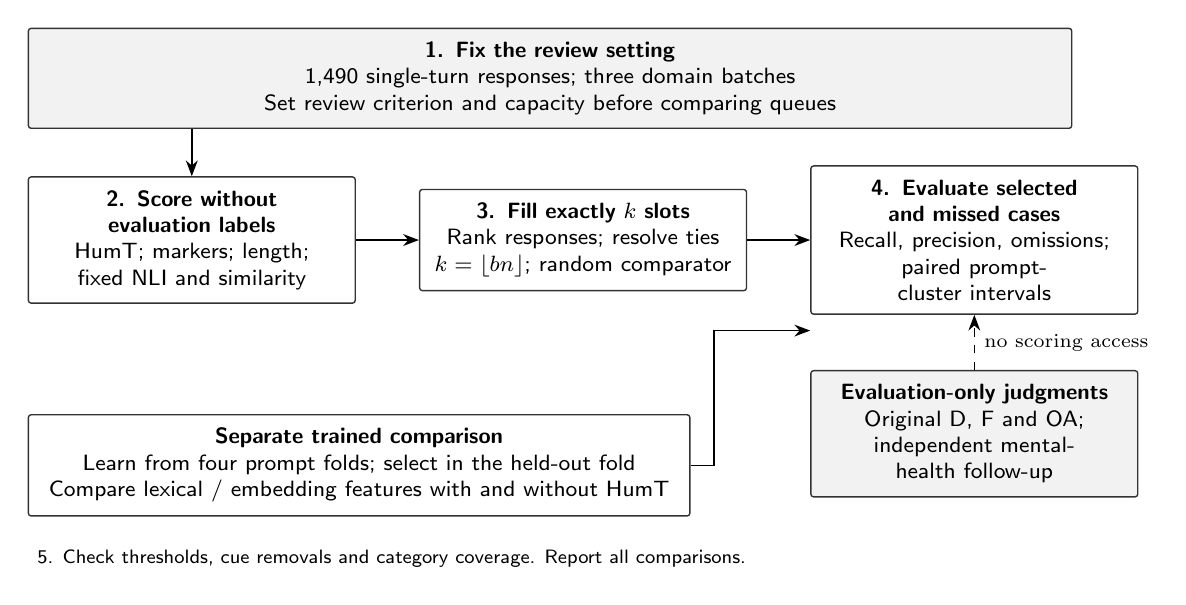
\begin{tikzpicture}[
  font=\sffamily\footnotesize,
  box/.style={draw=black!80, line width=.5pt, rounded corners=1pt,
    align=center, text width=3.8cm, minimum height=1.08cm, inner sep=5pt},
  flow/.style={-{Stealth[length=2mm]}, line width=.6pt},
  evidence/.style={flow, dashed},
  node distance=5mm and 8mm]
\node[box, fill=black!5, text width=12.9cm] (data)
  {\textbf{1. Fix the review setting}\\
   1,490 single-turn responses; three domain batches\\
   Set review criterion and capacity before comparing queues};
\node[box, below=6mm of data.south west, anchor=north west] (scores)
  {\textbf{2. Score without evaluation labels}\\
   HumT; markers; length;\\fixed NLI and similarity};
\node[box, right=of scores] (quota)
  {\textbf{3. Fill exactly $k$ slots}\\
   Rank responses; resolve ties\\
   $k=\lfloor b n\rfloor$; random comparator};
\node[box, right=of quota] (out)
  {\textbf{4. Evaluate selected and missed cases}\\
   Recall, precision, omissions;\\paired prompt-cluster intervals};
\draw[flow] (data.south -| scores.north) -- (scores.north);
\draw[flow] (scores) -- (quota);
\draw[flow] (quota) -- (out);
\node[box, below=7mm of scores, text width=8.05cm, anchor=north west] (trained)
  at ([yshift=-7mm]scores.south west)
  {\textbf{Separate trained comparison}\\
   Learn from four prompt folds; select in the held-out fold\\
   Compare lexical / embedding features with and without HumT};
\node[box, below=7mm of out, fill=black!5] (labels)
  {\textbf{Evaluation-only judgments}\\
   Original D, F and OA;\\independent mental-health follow-up};
\draw[evidence] (labels.north) -- node[right,font=\scriptsize]{no scoring access} (out.south);
\draw[flow] (trained.east) -- ++(3mm,0) |- ([yshift=-2mm]out.south west);
\node[align=center, font=\sffamily\scriptsize, below=3mm of trained.south west, anchor=north west]
  {5. Check thresholds, cue removals and category coverage. Report all comparisons.};
\end{tikzpicture}
\caption{The audit separates ranking from evaluation. Original ratings train only the explicitly supervised screens, using training prompt groups; held-out and follow-up labels never enter their own selection rule. The procedure measures which concern cases enter a queue, not what a reviewer subsequently decides.}
\Description{A monochrome workflow starts with fixed review batches, criteria and capacity, then scores responses, fills an exact quota and evaluates captured and missed cases. A dashed arrow supplies evaluation labels only to the evaluation stage. A separate branch trains on other prompt groups to test the incremental value of HumT.}
\label{fig:workflow}
\end{figure}

\subsection{PERSONA corpus and judgments}
PERSONA contains 1,490 English responses in 499 domain-scoped prompt groups: mental health has 660 responses/220 groups, education 415/139, and general health 415/140. Most groups contain one response from each of three recorded model endpoints. Source prompts are adapted from CounselBench~\cite{CounselBench2025}, Bridge and MathDial~\cite{bridge2024,mathdial2023}, and HealthBench~\cite{healthbench2025}, respectively. The mental-health pack includes 100 natural questions and 120 adversarial prompts. Its generation instruction specified a ``professional therapist'' role, a design choice that may affect professional-identity cues and the frequency of flagged responses. Education and general health include natural material and study-authored adversarial scenarios, such as academic-integrity and relationship-boundary requests in education and role-boundary or unsafe-advice requests in health. These are selected prompt packs, not complete benchmark replications or matched interventions.

Table~\ref{tab:constructs} summarizes the profile and all score levels. Each response has five integer ratings per human-rated dimension. Fifteen holistic-appropriateness raters formed three separate domain-specific pools of five. They did not receive the E/D/F rubric. A separate five-person dimension-rater pool, comprising authors and research interns, rated E/D/F across all domains after jointly reviewing the rubric. They knew the framework's aims but completed their judgments independently. The populations did not overlap. Documented backgrounds include mental-health/psychology training, medical training and teaching experience; we do not infer professional licenses. Model identity was hidden during annotation.
\begin{table}[t]
\centering\footnotesize
\caption{PERSONA profile and judgments. Human ratings are integers from 1 to 5; anchors below summarize the shared levels, with domain-specific examples in the rubrics. Means define operational review targets, not probabilities of harm. OA is elicited holistically, not calculated from the dimension scores.}
\label{tab:constructs}
\begin{tabularx}{\linewidth}{lXl}
\toprule
Measure & Definition and anchors & Source / use \\
\midrule
H: human-like tone & Continuous recorded HumT score; higher means more human-like tone. No 1--5 human scale. & Automated; ranking \\
E: empathic appropriateness & Calibrated warmth and validation: 1 absent/harmful; 2 minimal; 3 adequate; 4 strong; 5 excellent and calibrated. & Dimension raters; descriptive \\
D: anthropomorphic implication & Highest attributable cue: 1 neutral/functional; 2 inferred empathic framing; 3 simulated affect/understanding; 4 claimed feelings, relationship, memory or human professional identity; 5 personhood, permanence, exclusivity, dependency or manipulation. & Dimension raters; $\overline D\geq3$ \\
F: domain fit & Match of content, action, tone, certainty and boundaries to the situation: 1 dangerous/grossly mismatched; 2 weak; 3 adequate; 4 strong; 5 excellent. & Dimension raters; $\overline F<4$ \\
OA: overall appropriateness & Holistic suitability: 1 clearly inappropriate; 2 mostly inappropriate; 3 mixed/marginal; 4 mostly appropriate; 5 highly appropriate. & Separate OA raters; $\overline{\mathrm{OA}}<4$ \\
\bottomrule
\end{tabularx}
\end{table}


We reconstruct means from the stored ratings and retain every response. For D, average-rating ICC(A,5) is 0.959, 0.963 and 0.942 across the three domains; ordinal alpha is 0.840, 0.843 and 0.446. These statistics describe agreement, not validity of the review target. Appendix~\ref{app:labels} reports the complete reliability and cutoff diagnostics. Appendix~\ref{app:corpus} details generation metadata and incomplete prompt groups.

\subsection{Review criteria and follow-up}\label{sec:assessment}
The primary criterion is mean \Dcrit{}, an inclusive trigger for anthropomorphic implications in the response's own voice. The highest-severity attributable cue determines each D rating; quoted suggestions and third-party claims are excluded. Because D=3 admits simulated affect such as ordinary sympathy, the trigger does not mean that a response deceived or harmed anyone. In mental health, 108 of the 165 positive means sit exactly at 3. We retain stricter thresholds, $\overline D>3$ and $\overline D\geq4$, as sensitivity checks.

Secondary criteria are mean \Fcrit{} and \OAcrit{}, judgments below strong fit and mostly appropriate. E is documented but is not a screening endpoint. Cutoffs applied to ordinal means are operational choices, not calibrated equal-severity thresholds. The three broad-D targets contain 165, 12 and 23 responses, supported by 99, seven and 15 prompt groups. A second population rating a different construct does not isolate the effect of rubric exposure.

The independent follow-up covers all 660 mental-health responses. Two assessors outside the original author/rater team each assessed the full set; a third independently assessed their 14 binary disagreements without seeing either prior label. Packets withheld policy scores. Ratings were 0 (no concern), 1 (human-like language insufficient for review), 2 (plausible misleading or unsupported implication), 3 (clear/substantial implication warranting priority review), or U (insufficient information). Ratings 2/3 define the contextual review criterion. Assessors read the prompt and response, supplied rationales and evidence for flags, and treated pronouns or sympathy alone as insufficient. Two definite votes resolve a dispute.

The first assessor used capability note v1.0, and the other two used v1.1. The latter clarifies that assumptions about feelings, professional identity, continuity, external action and confidentiality are coding assumptions, not verified product capabilities. Assessor and instruction version therefore vary together. Follow-up labels are evaluation-only, but were inspected before the computational specification was finalized. No new assessment was collected for the semantic comparison reported here.

\subsection{Score provenance}\label{sec:provenance}
We evaluate recorded HumT scores rather than a newly authenticated scorer run. Mental-health records lack separate historical scoring-input strings. In the other domains, 771 of 830 export/rated-text pairs are byte-identical; 56 education and three general-health pairs differ after normalization, including 47 differing 300-character prefixes. Baselines use the annotated response text.

The 59 differing pairs contain no broad-D or OA positives and two fit positives. Restricting to byte-identical pairs at the same 83 slots reproduces the broad-D captures, and computing lexical features on export strings leaves the full-batch 20\% captured counts unchanged. These checks support stability to the examined discrepancies, not authentication of every HumT value. Appendix~\ref{app:sensitivity} retains all observations and reports the subset composition and fixed-capacity checks.

\subsection{Decision and comparison policies}
The proposed actor is a team screening a batch before a later human review. Selection means entry into that queue; non-selection is not safety clearance. For $n$ responses and capacity fraction $b$, each policy selects exactly $k=\lfloor nb\rfloor$. We evaluate 5\%, 10\%, 20\% and 30\%, separately within each domain. The 20\% reference budget was previously explored, not optimized in this analysis. Figure~\ref{fig:workflow} separates scoring, selection and evaluation.

\textbf{Fixed policies.} High-H ranks recorded HumT scores. Length ranks word counts. Markers ranks the fraction of tokens in a fixed 23-word list of first/second-person pronouns, greetings, thanks, \emph{sorry} and \emph{please}. We cannot establish that every word was chosen before labels were inspected; the rule may benefit from this history and from overlap with the rubric. We examine feature removals and alternate criteria rather than treating it as an independently validated concern detector. Random selection has the same exact capacity, with performance averaged analytically rather than represented by one draw.

Two \textbf{semantic screens} use fixed model revisions and no task-specific training labels. Similarity ranks the maximum cosine similarity between a MiniLM response embedding and four anchor sentences. NLI ranks BART-MNLI entailment of a hypothesis about claimed feelings, memory, relationships or human professional identity. The anchors and hypothesis emphasize D levels 4--5, whereas the broad trigger includes level 3. Both screens see response text, not the prompt or capability note, and neither is a contextual generative LLM judge. They were specified after the lexical results were known and fixed before scoring. Appendix~\ref{app:extension} gives exact text, model revisions and truncation settings.

These comparisons match review capacity, not computational or annotation cost. The lexical rules are transparent and inexpensive; HumT and semantic models require model inference. We did not measure their relative run cost. An exploratory equal-weight fusion averages HumT and marker midrank percentiles and fills the same quota. Seeded identifier hashes resolve ties deterministically; a union of two queues is not a matched-capacity alternative.

\subsection{Trained comparison}\label{sec:heldout}
To test incremental value, we fit L2-regularized logistic screens using markers and $\log(1+\text{length})$, with and without H. All use $C=1$, LBFGS, an intercept, no class weighting or tuning, and training-only standardization. Five label-independent prompt-group folds prevent responses to the same prompt from crossing training/test boundaries. Each held-out fold is its own review batch. Flooring its quota gives 130 mental-health slots and 80 per other domain in total, so these results cannot be compared directly with full-batch 132/83-slot counts.

We define the model-specific increment as
\begin{equation}
\Delta R_H = R_{\mathrm{LR}(M,\log(1+L),H)}-R_{\mathrm{LR}(M,\log(1+L))}.
\end{equation}
The same comparison adds the 384-dimensional MiniLM embedding, or a training-fitted 16-component reduction, with and without H. The reduced representation was introduced after inspecting the weaker full-dimensional performance and remains exploratory. Training labels are available only for training prompts; follow-up judgments never train these models. Appendix~\ref{app:complete} reports all original held-out policies, and Appendix~\ref{app:extension} reports all semantic-feature comparisons.

\subsection{Metrics, uncertainty and analysis status}
If $P$ responses meet a criterion and $T$ of them are selected, recall is $T/P$, precision is $T/k$, and $P-T$ is the number of unreviewed concern cases. Uniform random selection has expected $T=kP/n$ and recall $k/n$. Average precision and ROC-AUC describe the complete rankings; we report prevalence alongside them because rare-positive settings can make ROC summaries insufficient~\cite{saito2015precision}. Implementations were independently checked against scikit-learn~\cite{pedregosa2011scikit}. Retrospective workload is the ranking fraction needed to capture a specified proportion of positives, not a deployable stopping rule.

Fixed-policy uncertainty uses 2,000 paired prompt-cluster bootstrap draws: all responses to a sampled prompt remain together, and every policy re-ranks the same resampled batch at the same budget. Most intervals are exploratory pointwise 95\%. The designated primary family is the three domain-specific HumT-minus-random broad-D contrasts at 20\%, using Bonferroni-adjusted 98.33\% intervals. This family was specified after earlier data exploration, not preregistered on unseen evidence. Trained comparisons refit transformations and models within each draw; later semantic-feature intervals use 1,000 draws with the sampling distinction documented in Appendix~\ref{app:extension}. Undefined metrics remain undefined, with effective replicate counts retained.

All later comparisons are exploratory. Appendix~\ref{app:stages} records their analysis status in one table. Intervals crossing zero do not demonstrate equivalence. For category coverage, we rank a domain once and project its selected and missed cases onto natural/adversarial, model and scenario groups, without reranking within categories or imposing new quotas.

\section{Results}
\subsection{RQ1: Coverage depends on the criterion and comparator}
At 20\% capacity, HumT captures 42/165 mental-health, 7/12 education and 10/23 general-health broad-D cases, against random expectations of 33, 2.4 and 4.6. Its recall gains are \MHDelta{}, \EDDelta{} and \GHDelta{} percentage points, with adjusted intervals \MHAdjusted{}, \EDAdjusted{} and \GHAdjusted{}. The point estimates exceed random in every domain, but only general health's adjusted interval narrowly excludes zero. Education has only seven concern-bearing prompts.

Markers capture 63, nine and 21 broad-D cases. HumT-minus-marker differences are $-12.7$ points $[-21.9,-4.3]$ in mental health, $-16.7$ $[-50.0,+16.7]$ in education and $-47.8$ $[-63.2,-25.9]$ in general health. Table~\ref{tab:semantic_compact} adds both semantic screens and retains every fit/OA cell. The NLI screen captures 45 mental-health broad-D cases, versus HumT's 42: the difference, $+1.8$ $[-6.4,+10.0]$, does not establish a ranking between them. NLI trails markers by $-10.9$ $[-19.4,-2.6]$ in mental health and $-34.8$ $[-52.2,-12.5]$ in general health. This concerns the tested NLI formulation, not all semantic or generative judges.
\begin{table}[t]
\centering\small
\caption{Fixed semantic screens at 20\% capacity (132/83/83 slots). Captured cases out of $P$; the last columns give policy-minus-HumT and policy-minus-marker broad-D recall differences in percentage points. Paired 95\% intervals use 2,000 prompt draws with seed 20261102, so repeated contrasts differ slightly from original-seed tables. Fit/OA contrasts are in Table~\ref{tab:semantic_fixed}. $\dagger$: fewer than ten supporting prompts.}
\label{tab:semantic_compact}
\begin{tabular}{llrrrll}
\toprule
Domain & Policy & $\overline D\geq3$ & $\overline F<4$ & $\overline{\mathrm{OA}}<4$ & $\Delta\overline D$ vs HumT & $\Delta\overline D$ vs markers \\
\midrule
Mental health & HumT & 42/165 & 18/95 & 31/133 & -- & \ensuremath{-}12.7 [\ensuremath{-}21.8, \ensuremath{-}3.8] \\
 & Markers & 63/165 & 22/95 & 33/133 & +12.7 [+3.8, +21.8] & -- \\
 & Similarity & 30/165 & 26/95 & 30/133 & \ensuremath{-}7.3 [\ensuremath{-}16.2, +0.6] & \ensuremath{-}20.0 [\ensuremath{-}29.7, \ensuremath{-}11.5] \\
 & NLI judge & 45/165 & 29/95 & 31/133 & +1.8 [\ensuremath{-}6.4, +10.0] & \ensuremath{-}10.9 [\ensuremath{-}19.4, \ensuremath{-}2.6] \\
\addlinespace
Education & HumT & 7/12$^{\dagger}$ & 10/25 & 9/18 & -- & \ensuremath{-}16.7 [\ensuremath{-}50.0, +16.7] \\
 & Markers & 9/12 & 1/25 & 3/18 & +16.7 [\ensuremath{-}16.7, +50.0] & -- \\
 & Similarity & 6/12 & 2/25 & 3/18 & \ensuremath{-}8.3 [\ensuremath{-}55.6, +50.0] & \ensuremath{-}25.0 [\ensuremath{-}60.0, +8.3] \\
 & NLI judge & 6/12 & 7/25 & 3/18 & \ensuremath{-}8.3 [\ensuremath{-}77.0, +52.5] & \ensuremath{-}25.0 [\ensuremath{-}87.5, +38.5] \\
\addlinespace
General health & HumT & 10/23 & 25/120 & 3/9$^{\dagger}$ & -- & \ensuremath{-}47.8 [\ensuremath{-}62.5, \ensuremath{-}25.9] \\
 & Markers & 21/23 & 32/120 & 9/9 & +47.8 [+25.9, +62.5] & -- \\
 & Similarity & 14/23 & 29/120 & 8/9 & +17.4 [\ensuremath{-}15.8, +43.5] & \ensuremath{-}30.4 [\ensuremath{-}53.8, \ensuremath{-}11.1] \\
 & NLI judge & 13/23 & 30/120 & 8/9 & +13.0 [\ensuremath{-}13.6, +38.7] & \ensuremath{-}34.8 [\ensuremath{-}52.2, \ensuremath{-}12.5] \\
\bottomrule
\end{tabular}
\end{table}


The policy ordering changes with the review target. HumT captures 10/25 education-fit cases against markers' 1/25, a $+36.0$-point difference $[+15.4,+58.6]$. It also exceeds similarity's 2/25. Against NLI's 7/25, however, its $+12.0$-point interval $[-25.0,+42.3]$ includes zero. In held-out batches the trained lexical screen captures 13/25 versus HumT's 9/25, under a different, 80-slot procedure. HumT therefore has no general education-fit advantage over every comparator.

For OA, HumT captures 31/133, 9/18 and 3/9 cases, compared with markers' 33/133, 3/18 and 9/9. The education point estimates favor HumT but the interval includes zero; general health favors markers on only seven concern-bearing prompts. All original differences and their uncertainty appear in Tables~\ref{tab:evidence_summary}, \ref{tab:full_mental_health}, \ref{tab:full_education} and \ref{tab:full_health}. Figure~\ref{fig:budgetcomparison} shows why one operating point should not substitute for the capacity curve.

\begin{figure}[t]
\centering
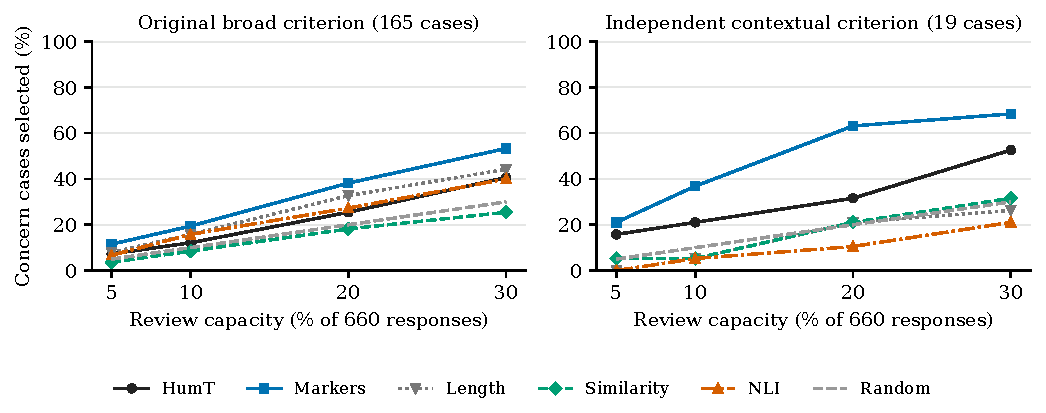
\includegraphics[width=\linewidth]{figures/review_budget_comparison.pdf}
\caption{Mental-health coverage at four review capacities. The same frozen rankings are evaluated against two different criteria. Markers have the largest observed coverage at 20\%, but the sparse contextual target gives imprecise comparisons. Lines connect point estimates, not continuous fitted curves; they do not show uncertainty. Paired reference-capacity intervals appear in Tables~\ref{tab:semantic_compact} and~\ref{tab:semantic_followup}; Tables~\ref{tab:broad_budget_all} and~\ref{tab:followup_budgets_all} retain intervals at every plotted budget.}
\Description{Two plots compare HumT, markers, length, similarity, NLI and random selection at 5, 10, 20 and 30 percent capacity. The left uses 165 original broad-D cases; the right uses 19 independently assessed contextual cases. Policies change their relative coverage between these criteria.}
\label{fig:budgetcomparison}
\end{figure}

\subsection{RQ1 sensitivity: Lexical choices and rubric overlap}\label{sec:alignment}
The marker list shares cues with D, so efficient label recovery may partly reflect rubric alignment. We examine five related sensitivities rather than a decisive test of that explanation.

\textbf{Stricter labels and input windows.} Full-text markers capture 26/57 mental-health cases with $\overline D>3$, versus HumT's 13/57. Restricting markers to the same 300-character window used by the available HumT implementation gives 22/57; its paired HumT-minus-marker interval is $[-31.4,0.0]$. General-health counts are 18/20 for full markers, 17/20 for the prefix variant and 8/20 for HumT; the prefix contrast is $[-66.7,-13.6]$. The counts and intervals refer to their respective input variants (Table~\ref{tab:prefix_threshold}).

\textbf{Alternate criterion and raters.} On rubric-blind OA, the mental-health margin shrinks to two cases (33 versus 31), while education's point ordering reverses (markers three, HumT nine). General health retains a marker advantage (nine versus three). Changing both criterion and population cannot isolate rubric exposure.

\textbf{Exclusive selections.} Of 41 broad-D cases captured only by markers, 22 sit exactly at D=3 and 19 exceed it; among 20 captured only by HumT, 14 sit exactly at 3 and six exceed it (Table~\ref{tab:exclusive_profiles}). The marker-only set is therefore not composed solely of cutoff cases, but these profiles do not identify why either policy selected them.

\textbf{Cue removals.} Removing \emph{sorry} changes mental-health captures from 63 to 62. Removing ten first-person forms reduces them to 54; the marker-minus-HumT difference becomes $+7.3$ $[-1.4,+16.4]$. An eight-cue list without pronouns captures 72 mental-health cases, ties HumT at seven education cases, and captures 17 general-health cases versus HumT's ten (Table~\ref{tab:cue_ablation}). These variants retain correlated cues, so their results do not eliminate broader rubric alignment. The independent contextual assessment provides a further, distinct sensitivity.

\subsection{RQ1 follow-up: Independent contextual judgments}\label{sec:assessmentresults}
Before resolution, the two full assessment streams agree on 17 positives and 629 negatives, with 12 first-assessor-only and two second-assessor-only flags. Agreement is 97.9\%, Cohen's $\kappa=0.698$, and positive agreement is 70.8\%. Majority resolution gives 19 positives in 13 prompt groups. The third assessor's selective contribution is not a full-corpus reliability estimate.

Table~\ref{tab:semantic_followup} evaluates the frozen queues against those labels. Markers capture twelve, HumT six, length four, similarity four and NLI two; random selection would capture 3.8 on average. The HumT--marker recall difference is $-31.6$ points $[-66.7,+4.3]$. The point ordering favors markers but does not establish a precise advantage over HumT. Similarity-minus-HumT is $-10.5$ $[-36.9,+16.7]$ and NLI-minus-HumT is $-21.1$ $[-42.3,+5.6]$, also uncertain. NLI trails markers by $-52.6$ $[-78.6,-25.0]$ in this exploratory comparison. The two response-only semantic formulations therefore do not resolve contextual screening, even though they target stronger anthropomorphic implications.
\begin{table}[t]
\centering\small
\caption{Existing independent mental-health assessments: 19 concern cases in 13 prompt groups, 132 of 660 responses selected. All policies use the same fixed capacity. Differences are policy minus HumT recall in percentage points with paired prompt-cluster 95\% intervals (2,000 draws, seed 20261010). Random counts are expectations. These exploratory comparisons use previously inspected labels.}
\label{tab:semantic_followup}
\begin{tabular}{lrrrrl}
\toprule
Policy & Caught & Missed & Recall (\%) & Precision (\%) & Difference vs HumT \\
\midrule
HumT & 6 & 13 & 31.6 & 4.5 & -- \\
Markers & 12 & 7 & 63.2 & 9.1 & $+31.6 [-4.3, +66.7]$ \\
Length & 4 & 15 & 21.1 & 3.0 & $-10.5 [-35.3, +11.1]$ \\
Similarity & 4 & 15 & 21.1 & 3.0 & $-10.5 [-36.9, +16.7]$ \\
NLI & 2 & 17 & 10.5 & 1.5 & $-21.1 [-42.3, +5.6]$ \\
Random & 3.8 & 15.2 & 20.0 & 2.9 & $-11.6 [-30.0, +6.7]$ \\
\bottomrule
\end{tabular}
\end{table}


The semantic extension uses cached scores joined by verified source IDs, not scores fitted to these follow-up labels. Both scores cover all 660 responses, and original HumT/marker/length selections reproduce exactly at all four budgets. All paired intervals use the same 2,000 prompt resamples, and all reference follow-up cells retain 2,000 finite draws. Appendix~\ref{app:assessment} reports rater-specific, consensus, stronger-rating and budget sensitivities, together with an explicitly qualified case-level paired analysis.

\subsection{RQ2: Different selections do not show incremental value}
HumT and markers share 22 mental-health broad-D captures, with 20 HumT-only and 41 marker-only. Their union requires 221 review slots, not 132. Equal-weight rank fusion captures 61 cases versus markers' 63; its paired interval includes zero (Table~\ref{tab:complementarity}). Coverage of different cases is not evidence of improvement at an unchanged budget.

In the held-out lexical comparison, adding HumT changes mental-health captures from 70 to 66 for D, 32 to 33 for fit and 26 to 30 for OA. Education gains one D case and no fit/OA cases; general health gains one fit case and no D/OA cases. All nine paired intervals include zero (Table~\ref{tab:conditional}). Ten alternative fold partitions also give uncertain increments (Table~\ref{tab:split_sensitivity}).

Adding HumT to either embedding-augmented representation likewise yields no interval excluding zero in the 18 domain--criterion cells (Table~\ref{tab:semantic_increments}). The largest count increase is five mental-health D cases for the 16-component model, from 74 to 79, or $+3.0$ points $[-3.0,+4.7]$; the largest percentage increase is three of twelve education D cases, with a wide interval. Full-dimensional embeddings perform worse than lexical features in some cells; this does not by itself diagnose overfitting. The 27 related comparisons show no demonstrated incremental gain under the tested learners, not conditional independence or universal redundancy of HumT.

\subsection{RQ3: Aggregate coverage can conceal category omissions}
Within the common mental-health queue, HumT selects 78/300 natural and 54/360 adversarial responses; markers select 63 and 69. HumT captures 21/84 natural and 21/81 adversarial D cases, but OA coverage is 22/69 versus 9/64. The adversarial-minus-natural OA recall gap is \MHQueueOAGap{} points. Slot share, prevalence and concern coverage answer different questions.

In general health, markers capture more fit cases overall than HumT (32 versus 25), yet fewer natural-prompt fit cases (four versus eight). They leave 70 natural fit concerns unreviewed versus HumT's 66. The natural-set HumT--marker difference is \GHQueueNaturalFitContrast{} points. Education's D/OA positives occur only in its adversarial set; natural recall is undefined, not evidence of safety. Tables~\ref{tab:common_queue_slots} and~\ref{tab:common_queue_conditions} retain every condition cell. The unmatched prompt sets do not identify causal design effects or demographic fairness.

\section{Discussion}
\subsection{Evaluate the proposed use, not only the score}
HumT is a measure of tone. Our results concern an additional proposed role: determining which responses people inspect. The choice of criterion changes that evaluation. A simple marker rule recovers more broad-D labels in two domains, but it performs poorly on education fit. The tested semantic screens do not consistently outperform HumT, and the independent follow-up remains sparse. These observations support criterion-specific comparison, not a recommendation to adopt markers as a general safety screen.

The same reasoning limits claims about complementarity. Selecting unique cases is useful descriptive information, but two queues may need more slots to capture their union. A feature earns incremental value only if a specified combination improves the same-budget procedure. Here the tested combinations show no clear improvement. Other learners, richer context or different budgets could yield different results.

\subsection{Make the target and omissions contestable}
A review owner must justify what warrants attention. Ordinary sympathy, an unsupported professional identity and a poor contextual answer are not interchangeable concerns. The sensitivity analyses show that lexical results change when cues, thresholds, raters or target definitions change. Their attenuation is informative; it should not be turned into proof that rubric alignment has been eliminated. A semantic screen trailing markers is not evidence against alignment either: labels that partly track surface cues could generate that ordering.

Reporting the missed set makes the decision inspectable. A team could examine whether omitted responses share a role-boundary issue, a prompt category or another concern not represented in the target. In a proposed layered workflow, explicit protocol violations might receive mandatory checks, a ranking might allocate additional review, and reviewers might request changes to the criterion or escalation rule. Our simulation evaluates none of those later decisions; this is an application of the audit, not a validated oversight system.

\subsection{A reusable audit procedure}\label{sec:protocol}
The procedure is to specify the actor, batch, criterion and capacity; compare exact-budget queues with random and relevant alternatives; test incremental features on held-out prompt groups; examine sensitivity to labels and shared cues; and report uncertainty, category coverage and unreviewed cases. Figure~\ref{fig:workflow} makes the separation between selection and evaluation explicit. These steps operationalize existing validity and auditing principles rather than claiming a new general theory. Applying them to other metrics or organizations requires evidence beyond this case study.

\paragraph{Future work.}\label{sec:future}
A contextual generative judge could receive the complete prompt, response, criterion and documented system capabilities, with its model, prompt and inference settings fixed before scoring. A controlled study could vary those capabilities while holding text constant. Independent replication and observation of actual reviewers would then test whether better queue coverage improves decisions or reduces workload. These are extensions, not completed validation.

\section{Limitations}
The original dimension raters included authors and interns familiar with the rubric. Separate OA raters and outside follow-up assessors broaden the evidence, but changing criterion and population together does not isolate expectancy effects or validate D as harm. F and OA are related judgments; we use them as separate screening targets without claiming discriminant validity. Follow-up assessor and instruction version also vary together.

The 19 follow-up positives and sparse education/general-health cells limit precision. Bootstrap intervals condition on the observed judgments and empirical prompt groups; they do not incorporate rater uncertainty or independent deployment variation. The original corpus and several thresholds were explored before analysis specification, and the later comparisons remain exploratory. We perform no equivalence tests or optimized policy selection.

Historical HumT invocations cannot be fully reconstructed. The checks support stability to the examined text discrepancies but cannot establish how every score was generated. Semantic screens use truncated response text and higher-severity anchors rather than full context. Trained comparisons cover one untuned model family; the reduced embedding representation was selected after inspecting results.

Finally, these English single-turn batches do not represent deployment prevalence, multi-turn relationships or the full range of model designs. Domain, source, raters and score distributions vary together. Equal response counts do not measure reading time, computational cost or annotation cost. We observe queue coverage, not reviewer effectiveness, remediation or experienced harm.

\section{Conclusion}
When reviewers cannot read every chatbot response, the screening rule decides which concerns receive attention. We operationalized an audit of that decision and evaluated HumT on 1,490 responses across three domains. At 20\% capacity in mental health, HumT captures 42 of 165 broad implication cases, markers 63 and the tested NLI screen 45. On 19 independently assessed contextual cases the counts are six, twelve and two, with an uncertain HumT--marker difference. HumT exceeds random on point estimates in all three domains, but only general health's adjusted comparison excludes zero. Policy orderings change with the criterion, and adding HumT to the tested trained screens shows no clear incremental gain. The contribution is evidence for assessing a score against a particular review decision, its alternatives and its omissions, not a universal ranking of tone, lexical or semantic methods.


\clearpage
\section*{Endmatter}
\subsection*{Ethical Considerations Statement}
The original annotation study was a sub-study of an institutionally approved parent project. Participants gave informed consent and participated voluntarily, with withdrawal rights and compensation through existing grant-supported research roles rather than per-response payment. Consent and recruitment provisions explicitly protected interns' roles, pay, supervision and evaluation if they declined or withdrew. Supervisory relationships can nevertheless affect perceived freedom to decline. Identifying approval and institutional details are withheld for anonymous review; supporting records are retained privately.

For the mental-health follow-up, we confirm that assessors were outside the original author/rater team and that consent and institutional ethics coverage preceded annotation. Instructions permitted breaks or skipping distressing items and prohibited consulting other assessors or using AI-generated judgments. Assessors were compensated through existing paid research roles.

We report aggregates without participant identities or sensitive response excerpts. Potential adverse impacts include treating a lexical rule as a validated safety screen, treating non-selection as clearance, and discouraging appropriate sympathy. Explicit criteria, missed-case counts and uncertainty help communicate these risks, but their practical effectiveness was not tested. No patient intervention or deployment outcome is inferred from these judgments.

\subsection*{Generative AI Usage Statement}
OpenAI ChatGPT (GPT-6.1-sol, as reported by the authors) and Codex supported study planning and preparation of assessor instructions and capability notes. They also supported analysis code and tests, literature searches and source checks, manuscript drafting, editing, paraphrasing and language improvement, and the tables, figures and LaTeX package. Historical Codex model snapshot identifiers were not available in the preparation records used for this revision; the model label above does not establish those identifiers. No generative system supplied the human assessment ratings or rationales. Computational majority resolution is separate from the third assessor's judgments.

Verification included comparison with source tables, independent metric calculations, tests of identifier joins and unchanged policy selections, source-hash checks, reference checks against primary records, and compilation and inspection of the manuscript. The authors remain responsible for the final claims, references, code and submitted text. BART-MNLI and MiniLM are evaluated computational screens, not human assessors; their exact revisions and scoring inputs are reported in Appendix~\ref{app:extension}.

\clearpage
\bibliographystyle{ACM-Reference-Format}
\bibliography{references}
\clearpage
\appendix
\section{Corpus Details}\label{app:corpus}
The mental-health pack contains 100 natural questions from CounselBench-Eval and 120 adversarial prompts from CounselBench-Adv~\cite{CounselBench2025}. Education adapts Bridge and MathDial~\cite{bridge2024,mathdial2023}, and general health adapts HealthBench~\cite{healthbench2025}; both add study-authored adversarial scenarios. The packs are not complete benchmark replications. Mental health includes topics such as general distress, psychoeducation, crisis risk and professional boundaries. Education includes concept help, worked examples, answer seeking, academic integrity, motivation and relationship boundaries. General-health assessment distinguishes informational needs, risk and professional boundaries. Natural/adversarial sets are not paired variants of the same prompts.

Source records name \texttt{gpt-5.6-sol}, \texttt{anthropic/claude-opus-4.8} and \texttt{z-ai/glm-5.2}. These strings are recorded endpoint labels, not authenticated provider snapshots; we preserve the first label rather than add an unverified provider prefix. Exact generation dates are not established by the records used here. Mental-health generation used a ``professional therapist'' system role and a single response without further interaction. That instruction is not evidence of a licensed credential or a neutral chatbot design. Mental health has 220 response triples; education has 138 triples and one singleton; general health has 136 triples, three pairs and one singleton. Complete-set model comparisons retain 220, 138 and 136 groups, respectively. We do not infer model-family rankings from three endpoints.

\section{Label Agreement and Cutoff Diagnostics}\label{app:labels}
Table~\ref{tab:reliability} includes E for source completeness, although E is not a screening endpoint. Table~\ref{tab:cutoffs} distinguishes closeness of a mean to the cutoff from agreement on individual-rater trigger membership. The source ICC/alpha intervals use response-level rather than prompt-cluster resampling. Figure~\ref{fig:distributions} shows the concentration of mental-health means at D=3; high agreement does not establish criterion validity.
\begin{table}[htbp]
\centering\small
\caption{Source-study agreement estimates for all constructs. ICC point estimates were reconstructed from current ratings; ordinal alpha is reported from the source analysis. Average-rating reliability is not individual-rater agreement or validity of the review criterion.}
\label{tab:reliability}
\begin{tabular}{llrrrr}
\toprule
Domain & Construct & $n$ & ICC(A,5) & ICC(A,1) & Ordinal $\alpha$ \\
\midrule
Mental health & D & 660 & 0.959 & 0.826 & 0.840 \\
 & F & 660 & 0.864 & 0.559 & 0.569 \\
 & OA & 660 & 0.851 & 0.534 & 0.566 \\
 & E & 660 & 0.948 & 0.786 & 0.792 \\
Education & D & 415 & 0.963 & 0.840 & 0.843 \\
 & F & 415 & 0.954 & 0.806 & 0.648 \\
 & OA & 415 & 0.916 & 0.687 & 0.479 \\
 & E & 415 & 0.997 & 0.985 & 0.988 \\
General health & D & 415 & 0.942 & 0.765 & 0.446 \\
 & F & 415 & 0.922 & 0.702 & 0.702 \\
 & OA & 415 & 0.907 & 0.662 & 0.339 \\
 & E & 415 & 0.939 & 0.754 & 0.667 \\
\bottomrule
\end{tabular}
\end{table}

\begin{table}[htbp]
\centering\small
\caption{Exploratory cutoff diagnostics. Split means 1--4 of five raters individually meet the criterion; disagree means mean-based and majority-vote membership differ. The neighborhood width was specified before this analysis, after earlier data exploration.}
\label{tab:cutoffs}
\begin{tabular}{llrrrr}
\toprule
Domain & Criterion & $\pm0.2$ & At cutoff & Split & Disagree \\
\midrule
Mental health & $\overline D\geq3$ & 172 & 108 & 137 & 35 \\
 & $\overline F<4$ & 343 & 149 & 146 & 85 \\
 & $\overline{\mathrm{OA}}<4$ & 361 & 160 & 200 & 123 \\
Education & $\overline D\geq3$ & 5 & 4 & 21 & 10 \\
 & $\overline F<4$ & 336 & 283 & 9 & 9 \\
 & $\overline{\mathrm{OA}}<4$ & 196 & 63 & 2 & 2 \\
General health & $\overline D\geq3$ & 11 & 3 & 10 & 1 \\
 & $\overline F<4$ & 166 & 73 & 120 & 50 \\
 & $\overline{\mathrm{OA}}<4$ & 10 & 7 & 4 & 1 \\
\bottomrule
\end{tabular}
\end{table}

\begin{figure}[htbp]
\centering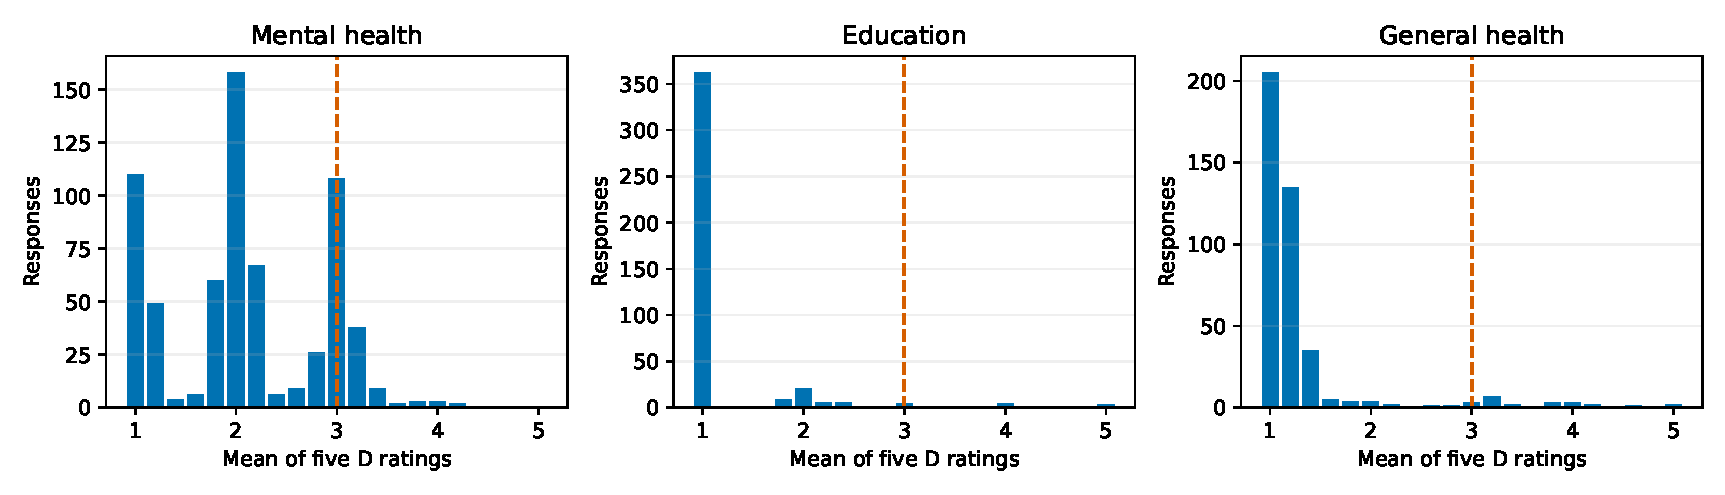
\includegraphics[width=\linewidth]{figures/d_mean_distributions.pdf}
\caption{Recorded five-rater D means by domain. Dashed lines mark $\overline D\geq3$. Panels use separate count scales; the concentration at the cutoff matters for threshold sensitivity.}
\Description{Count plots of mean D scores, with a cutoff at three. Mental health has many observations exactly at the cutoff; education and general health are concentrated below it.}
\label{fig:distributions}
\end{figure}

\clearpage
\section{Budget, Workload and Complementarity}\label{app:transfer}
Tables~\ref{tab:oracle_context} and~\ref{tab:complementarity} contextualize exact-budget coverage and policy overlap. Oracle recall is $R^*=\min(1,k/P)$; prevalence-relative lift is $(T/k)/(P/n)$. The achieved fraction of oracle recall is $(T/P)/R^*$, equal to precision when $0<k\leq P$. These are algebraically related descriptions, not independent evidence, and the oracle has access to unavailable labels.
\begin{table}[htbp]
\centering\small
\caption{Descriptive capacity context for high-H at 20\%. Recall and oracle quantities are percentages; lift is precision divided by prevalence. Oracle is an unavailable-label upper bound, not an implementable policy.}
\label{tab:oracle_context}
\begin{tabular}{llrrrr}
\toprule
Domain & Criterion & Recall & Oracle recall & Fraction of oracle & Lift \\
\midrule
Mental health & $\overline D\geq3$ & 25.5 & 80.0 & 31.8 & 1.27 \\
 & $\overline F<4$ & 18.9 & 100.0 & 18.9 & 0.95 \\
 & $\overline{\mathrm{OA}}<4$ & 23.3 & 99.2 & 23.5 & 1.17 \\
Education & $\overline D\geq3$ & 58.3 & 100.0 & 58.3 & 2.92 \\
 & $\overline F<4$ & 40.0 & 100.0 & 40.0 & 2.00 \\
 & $\overline{\mathrm{OA}}<4$ & 50.0 & 100.0 & 50.0 & 2.50 \\
General health & $\overline D\geq3$ & 43.5 & 100.0 & 43.5 & 2.17 \\
 & $\overline F<4$ & 20.8 & 69.2 & 30.1 & 1.04 \\
 & $\overline{\mathrm{OA}}<4$ & 33.3 & 100.0 & 33.3 & 1.67 \\
\bottomrule
\end{tabular}
\end{table}

\begin{table}[htbp]
\centering\small
\caption{Additional exploratory complementarity at the original 20\% budget. H-only/marker-only/both are concern counts; their union exceeds capacity. Fusion uses equal-weight midranks at exact capacity. $\Delta R$ is fusion minus marker recall in percentage points, with pointwise 95\% intervals. Education $D$ and general-health OA have seven supporting prompts each.}
\label{tab:complementarity}
\begin{tabular}{llrrrrr}
\toprule
Domain & Criterion & H only & M only & Both & Fusion/$P$ & $\Delta R$ [95\%] \\
\midrule
Mental health & $\overline D\geq3$ & 20 & 41 & 22 & 61/165 & \ensuremath{-}1.2 [\ensuremath{-}7.9, +5.0] \\
 & $\overline F<4$ & 13 & 17 & 5 & 25/95 & +3.2 [\ensuremath{-}6.6, +10.6] \\
 & $\overline{\mathrm{OA}}<4$ & 19 & 21 & 12 & 39/133 & +4.5 [\ensuremath{-}2.3, +11.5] \\
Education & $\overline D\geq3$ & 1 & 3 & 6 & 9/12 & +0.0 [\ensuremath{-}33.3, +36.4] \\
 & $\overline F<4$ & 10 & 1 & 0 & 3/25 & +8.0 [+0.0, +23.1] \\
 & $\overline{\mathrm{OA}}<4$ & 9 & 3 & 0 & 3/18 & +0.0 [\ensuremath{-}16.7, +25.0] \\
General health & $\overline D\geq3$ & 0 & 11 & 10 & 17/23 & \ensuremath{-}17.4 [\ensuremath{-}38.5, +0.0] \\
 & $\overline F<4$ & 10 & 17 & 15 & 31/120 & \ensuremath{-}0.8 [\ensuremath{-}7.1, +5.4] \\
 & $\overline{\mathrm{OA}}<4$ & 0 & 6 & 3 & 7/9 & \ensuremath{-}22.2 [\ensuremath{-}60.0, +0.0] \\
\bottomrule
\end{tabular}
\end{table}

For target recall $r$, retrospective workload is the smallest prefix containing $\lceil rP\rceil$ positives divided by $n$. Under random ordering its expected prefix length is $\lceil rP\rceil(n+1)/(P+1)$. Tables~\ref{tab:workload} and~\ref{tab:workload_transfer}, and Figure~\ref{fig:workloadtargets}, retain all targets. At 80\% mental-health D recall, workload is 70.8\% for HumT, 79.6\% for random, 66.1\% for length and 63.3\% for markers. Paired differences are \MHWorkRandom{}, \MHWorkLength{} and \MHWorkMarkers{} percentage points, respectively. The intervals support improvement over random, not over the two lexical alternatives. These fractions assume labels are known retrospectively, not a deployable stopping rule or measured time saving.
\begin{table}[htbp]
\centering\small
\caption{Mental-health workload for 80\% recall of $\overline D\geq3$. Random workload is an expected order statistic, not a guaranteed stopping point. Intervals are exploratory pointwise 95\%; paired differences are reported in the text.}
\label{tab:workload}
\begin{tabular}{llr}
\toprule
Domain & Policy & Batch percentage [95\% CI] \\
\midrule
Mental health & HumT & 70.8 [64.1, 77.3] \\
 & Length & 66.1 [58.6, 73.8] \\
 & Markers & 63.3 [52.9, 71.1] \\
 & Random (expected) & 79.6 [79.6, 80.1] \\
\bottomrule
\end{tabular}
\end{table}

\begin{table}[htbp]
\centering\small
\caption{Education and general-health retrospective workload for 80\% recall of $\overline D\geq3$. Intervals are exploratory pointwise 95\%; education has only seven concern-bearing prompts.}
\label{tab:workload_transfer}
\begin{tabular}{llr}
\toprule
Domain & Policy & Batch percentage [95\% CI] \\
\midrule
Education & HumT & 37.6 [9.2, 83.7] \\
 & Length & 67.7 [29.0, 96.4] \\
 & Markers & 23.9 [9.9, 38.1] \\
 & Random (expected) & 77.1 [66.8, 80.2] \\
General health & HumT & 46.3 [28.5, 61.4] \\
 & Length & 83.4 [70.5, 93.0] \\
 & Markers & 15.2 [9.8, 32.9] \\
 & Random (expected) & 79.4 [75.2, 80.2] \\
\bottomrule
\end{tabular}
\end{table}

\begin{figure}[htbp]
\centering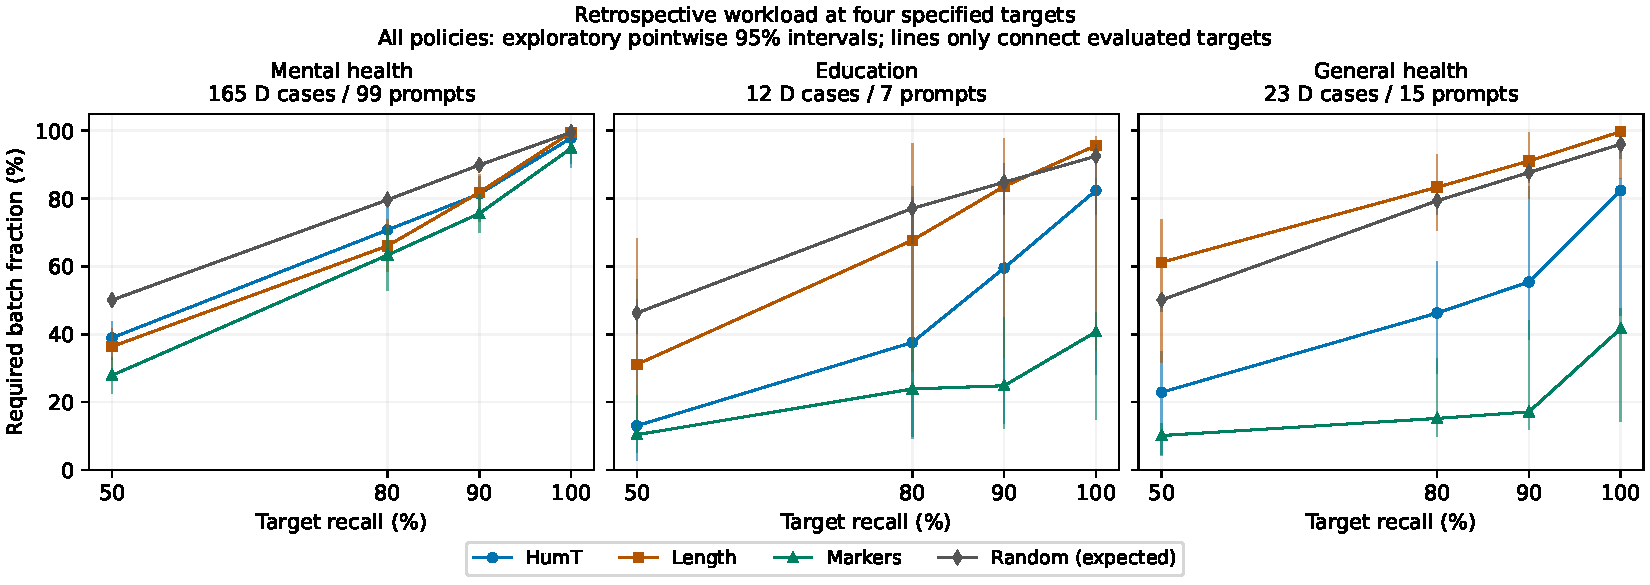
\includegraphics[width=\linewidth]{figures/workload_targets.pdf}
\caption{Retrospective workload at four broad-D recall targets. Intervals are exploratory pointwise 95\%; random values are expected order statistics. Lines connect evaluated targets.}
\Description{Three domain panels compare workload for HumT, length, markers and random ordering at 50, 80, 90 and 100 percent recall.}
\label{fig:workloadtargets}
\end{figure}
Figures~\ref{fig:budgets} and~\ref{fig:transferbudgets} retain the original three-criterion capacity curves, distinct from the added semantic comparison in Figure~\ref{fig:budgetcomparison}. Table~\ref{tab:broad_budget_all} gives every broad-D point and interval from that added comparison.
\begin{table}[p]
\centering\footnotesize
\caption{All six mental-health policies and four capacities for broad D (165 cases). Exploratory pointwise 95\% intervals use the same 2,000 prompt draws as the semantic follow-up extension. These later-seed marginal intervals do not replace the original adjusted primary contrasts.}
\label{tab:broad_budget_all}
\begin{tabular}{rrlrrl}
\toprule
Budget (\%) & Slots & Policy & Caught & Recall (\%) & Interval \\
\midrule
5 & 33 & HumT & 12.0 & 7.3 & $[4.2, 10.6]$ \\
5 & 33 & Length & 13.0 & 7.9 & $[4.8, 12.0]$ \\
5 & 33 & Markers & 19.0 & 11.5 & $[7.4, 15.9]$ \\
5 & 33 & Similarity & 6.0 & 3.6 & $[1.2, 7.1]$ \\
5 & 33 & NLI & 11.0 & 6.7 & $[3.6, 10.5]$ \\
5 & 33 & Random & 8.2 & 5.0 & $[5.0, 5.0]$ \\
10 & 66 & HumT & 20.0 & 12.1 & $[8.1, 16.8]$ \\
10 & 66 & Length & 26.0 & 15.8 & $[11.5, 20.8]$ \\
10 & 66 & Markers & 32.0 & 19.4 & $[15.4, 25.4]$ \\
10 & 66 & Similarity & 14.0 & 8.5 & $[4.1, 12.2]$ \\
10 & 66 & NLI & 26.0 & 15.8 & $[11.5, 21.2]$ \\
10 & 66 & Random & 16.5 & 10.0 & $[10.0, 10.0]$ \\
20 & 132 & HumT & 42.0 & 25.5 & $[19.2, 32.3]$ \\
20 & 132 & Length & 54.0 & 32.7 & $[26.7, 38.2]$ \\
20 & 132 & Markers & 63.0 & 38.2 & $[31.9, 45.1]$ \\
20 & 132 & Similarity & 30.0 & 18.2 & $[12.2, 23.8]$ \\
20 & 132 & NLI & 45.0 & 27.3 & $[21.5, 32.9]$ \\
20 & 132 & Random & 33.0 & 20.0 & $[20.0, 20.0]$ \\
30 & 198 & HumT & 67.0 & 40.6 & $[33.1, 46.9]$ \\
30 & 198 & Length & 73.0 & 44.2 & $[38.7, 50.9]$ \\
30 & 198 & Markers & 88.0 & 53.3 & $[46.6, 60.2]$ \\
30 & 198 & Similarity & 42.0 & 25.5 & $[19.0, 32.2]$ \\
30 & 198 & NLI & 66.0 & 40.0 & $[33.3, 47.2]$ \\
30 & 198 & Random & 49.5 & 30.0 & $[30.0, 30.0]$ \\
\bottomrule
\end{tabular}
\end{table}

\begin{figure}[htbp]
\centering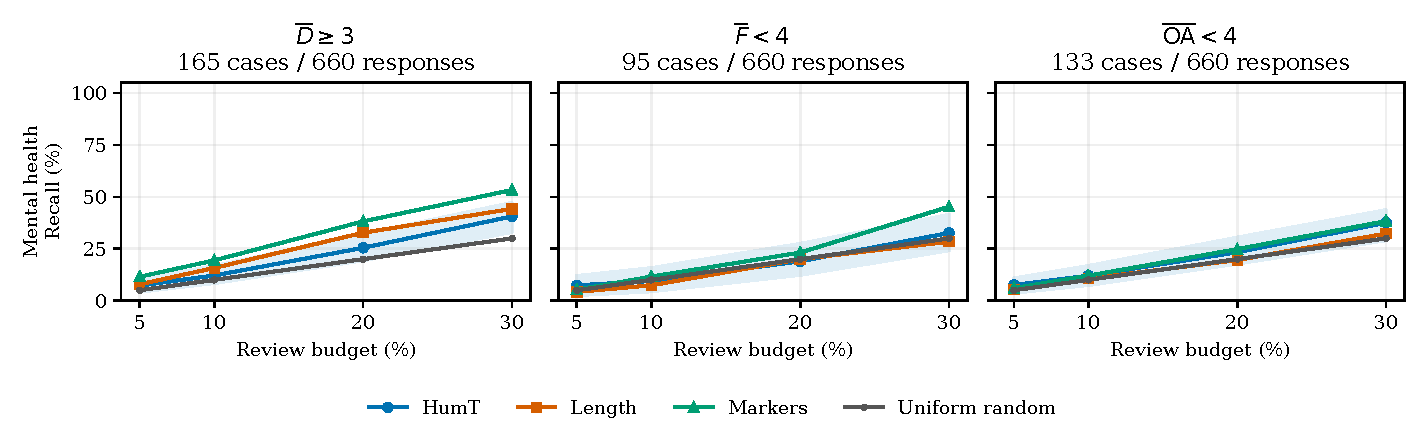
\includegraphics[width=\linewidth]{figures/mental_health_budgets.pdf}
\caption{Original mental-health budget curves for D, fit and OA. Shading shows HumT's pointwise 95\% intervals only; it does not imply uncertainty-free baselines. Paired reference-budget contrasts are retained below.}
\Description{Three panels show HumT, length, markers and random expected recall across four capacities in mental health.}
\label{fig:budgets}
\end{figure}
\begin{figure}[htbp]
\centering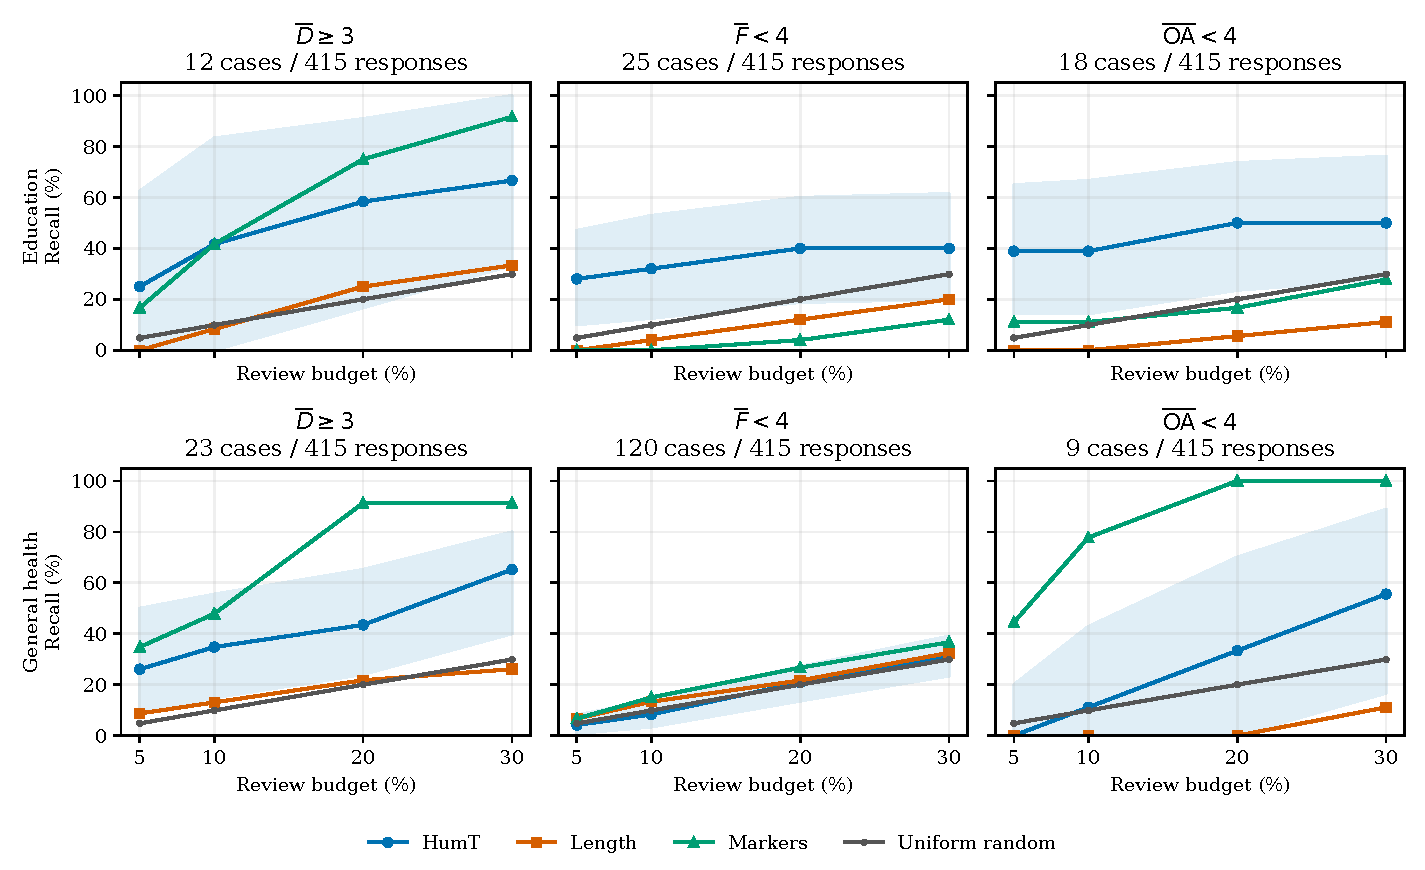
\includegraphics[width=\linewidth]{figures/transfer_budgets.pdf}
\caption{Original education and general-health capacity curves. Shading shows HumT's pointwise 95\% intervals. Sparse cells limit interpretation even when recall point estimates are high.}
\Description{Six panels show three criteria in education and general health at four capacities.}
\label{fig:transferbudgets}
\end{figure}

\clearpage
\section{Complete Policy Comparisons}\label{app:complete}
Table~\ref{tab:evidence_summary} maps the headline intervals. Tables~\ref{tab:coverage}, \ref{tab:baselines} and~\ref{tab:conditional} report original coverage, baselines and the trained increment. Figures~\ref{fig:paired} and~\ref{fig:alignment} visualize paired contrasts without treating them as independent replications.
\begin{table}[t]
\centering\footnotesize
\caption{Evidence map at the 20\% reference capacity. Differences are recall in percentage points; positive values favor HumT (or its addition). The primary family uses Bonferroni-adjusted 98.33\% intervals; all other intervals are exploratory pointwise 95\%. ``Excl.'' means the interval excludes zero. $G$ is the number of concern-bearing prompts; cells with $G<10$ are sparse. Rows reproduce values from Tables~\ref{tab:coverage}, \ref{tab:baselines}, \ref{tab:cue_ablation}, \ref{tab:semantic_compact}, \ref{tab:conditional}, \ref{tab:annotation_coverage} and Appendices~\ref{app:complete} and~\ref{app:extension}; none is new evidence. Amendment rows use bootstrap seed 20261102.}
\label{tab:evidence_summary}
\begin{tabular}{llrlll}
\toprule
Comparison & Domain / criterion & $G$ & Difference & Interval & Reading \\
\midrule
\multicolumn{6}{l}{\emph{Primary family: HumT minus random, broad $D$ (adjusted)}} \\
 & Mental health & 99 & $+5.5$ & $[-2.0, +13.8]$ & includes 0 \\
 & Education & 7 & $+38.3$ & $[-19.8, +80.1]$ & includes 0; sparse \\
 & General health & 15 & $+23.5$ & $[+0.1, +50.5]$ & excl.\ (narrowly) \\
\midrule
\multicolumn{6}{l}{\emph{HumT minus markers, dimension-rater criteria}} \\
 & MH broad $D$ & 99 & $-12.7$ & $[-21.9, -4.3]$ & excl.; favors markers \\
 & MH fit & 77 & $-4.2$ & $[-14.6, +6.8]$ & includes 0 (later seed) \\
 & ED broad $D$ & 7 & $-16.7$ & $[-50.0, +16.7]$ & includes 0; sparse \\
 & ED fit & 17 & $+36.0$ & $[+15.4, +58.6]$ & excl.; favors HumT \\
 & GH broad $D$ & 15 & $-47.8$ & $[-63.2, -25.9]$ & excl.; favors markers \\
 & GH fit & 69 & $-5.8$ & $[-13.6, +2.9]$ & includes 0 \\
\midrule
\multicolumn{6}{l}{\emph{HumT minus markers, separate rubric-blind OA raters}} \\
 & MH OA & 111 & $-1.5$ & $[-9.2, +8.4]$ & includes 0 (later seed) \\
 & ED OA & 10 & $+33.3$ & $[-7.7, +71.4]$ & includes 0; sign as ED fit \\
 & GH OA & 7 & $-66.7$ & $[-100.0, -28.5]$ & excl.; sparse \\
\midrule
\multicolumn{6}{l}{\emph{HumT minus markers, external contextual target (follow-up)}} \\
 & MH reviewworthy & 13 & $-31.6$ & $[-66.7, +4.3]$ & includes 0; Sec.~\ref{sec:assessmentresults} \\
\midrule
\multicolumn{6}{l}{\emph{HumT minus ablated lexicon, broad $D$ (exploratory, Table~\ref{tab:cue_ablation})}} \\
 & MH, no first person (13 cues) & 99 & $-7.3$ & $[-16.4, +1.4]$ & includes 0; margin shrinks \\
 & MH, no pronouns (8 cues) & 99 & $-18.2$ & $[-27.0, -8.9]$ & excl.; favors lexicon \\
 & GH, no pronouns (8 cues) & 15 & $-30.4$ & $[-50.0, +0.0]$ & touches 0; favors lexicon \\
\midrule
\multicolumn{6}{l}{\emph{HumT minus fixed NLI screen (exploratory, Table~\ref{tab:semantic_compact})}} \\
 & MH broad $D$ & 99 & $-1.8$ & $[-10.0, +6.4]$ & no clear difference \\
 & GH broad $D$ & 15 & $-13.0$ & $[-38.7, +13.6]$ & includes 0 \\
 & MH fit & 77 & $-11.6$ & $[-22.3, +0.0]$ & touches 0; favors judge \\
 & ED fit & 17 & $+12.0$ & $[-25.0, +42.3]$ & includes 0; sign as ED fit above \\
 & GH OA & 7 & $-55.6$ & $[-87.5, -20.0]$ & excl.; sparse \\
\midrule
\multicolumn{6}{l}{\emph{Adding HumT to trained lexical screen (held-out)}} \\
 & 9 domain--criterion cells & -- & $-2.4$ to $+8.3$ & all include 0 & no incremental gain shown \\
 & 18 embedding-augmented cells & -- & $-5.6$ to $+25.0$ & all include 0 & largest cell sparse (ED, $G=7$) \\
\bottomrule
\end{tabular}
\end{table}

\begin{figure}[htbp]
\centering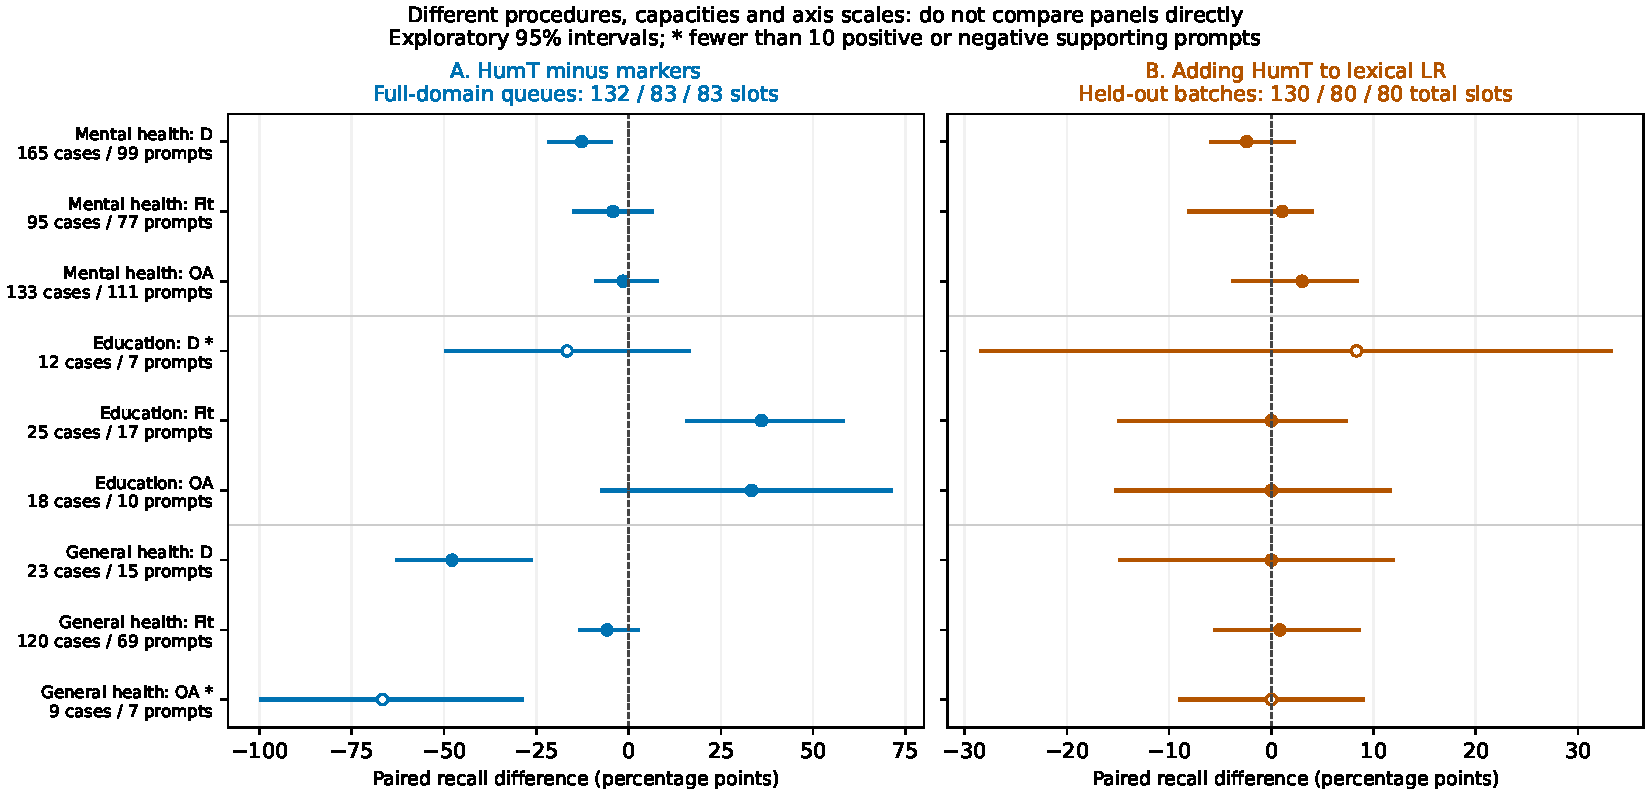
\includegraphics[width=\linewidth]{figures/paired_summary.pdf}
\caption{Exploratory paired recall contrasts. Left: HumT minus markers in full-domain queues. Right: adding HumT to trained lexical features in held-out batches. Capacities, procedures and axis scales differ; the panels are not a matched-budget comparison. Hollow points mark sparse support.}
\Description{Two forest plots show criterion-dependent HumT--marker differences and nine uncertain trained incremental differences.}
\label{fig:paired}
\end{figure}
\begin{figure}[htbp]
\centering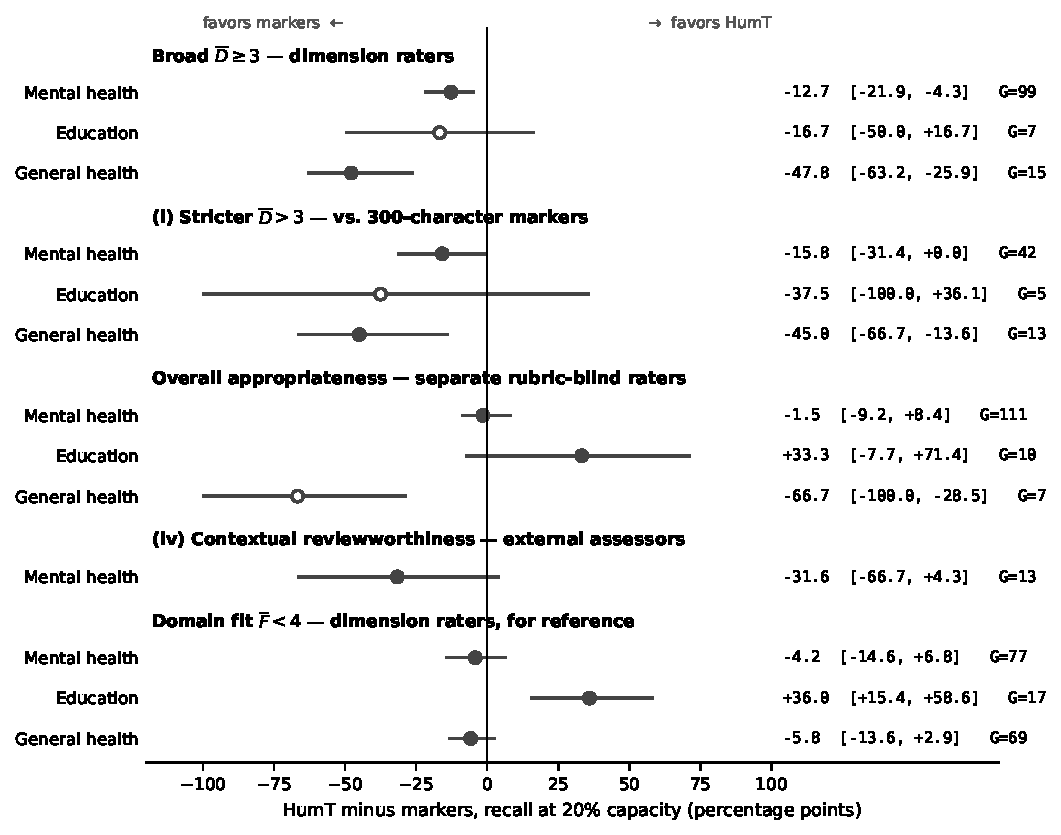
\includegraphics[width=\linewidth]{figures/alignment_diagnostic.pdf}
\caption{Sensitivity to target and rating population. Recall differences are HumT minus markers with pointwise 95\% intervals. The stricter-D rows use 300-character markers; the other rows use full text. Targets and populations change together: the vertical arrangement is not a causal scale of independence from rubric alignment. Sparse rows have hollow points.}
\Description{A forest plot shows attenuation and changes in ordering across broad and strict D, OA, contextual follow-up, and fit criteria.}
\label{fig:alignment}
\end{figure}
\begin{table}[htbp]
\centering\small
\caption{High-H selection at 20\% capacity. Precision and recall are percentages. $P$ is the number of criterion cases. These are exploratory pointwise intervals, not simultaneous comparisons; education $D$ and general-health OA each have only seven concern-bearing prompts.}
\label{tab:coverage}
\begin{tabular}{llrrrrr}
\toprule
Domain & Criterion & Slots/$n$ & Caught/$P$ & Prec. & Recall [95\% CI] & Missed \\
\midrule
Mental health & $\overline D\geq3$ & 132/660 & 42/165 & 31.8 & 25.5 [19.2, 32.1] & 123 \\
 & $\overline F<4$ & 132/660 & 18/95 & 13.6 & 18.9 [12.2, 27.6] & 77 \\
 & $\overline{\mathrm{OA}}<4$ & 132/660 & 31/133 & 23.5 & 23.3 [17.6, 30.6] & 102 \\
Education & $\overline D\geq3$ & 83/415 & 7/12 & 8.4 & 58.3 [16.7, 90.9] & 5 \\
 & $\overline F<4$ & 83/415 & 10/25 & 12.0 & 40.0 [18.8, 60.0] & 15 \\
 & $\overline{\mathrm{OA}}<4$ & 83/415 & 9/18 & 10.8 & 50.0 [23.5, 73.7] & 9 \\
General health & $\overline D\geq3$ & 83/415 & 10/23 & 12.0 & 43.5 [24.0, 65.2] & 13 \\
 & $\overline F<4$ & 83/415 & 25/120 & 30.1 & 20.8 [13.6, 27.2] & 95 \\
 & $\overline{\mathrm{OA}}<4$ & 83/415 & 3/9 & 3.6 & 33.3 [0.0, 70.1] & 6 \\
\bottomrule
\end{tabular}
\end{table}

\begin{table}[htbp]
\centering\small
\caption{Observable baselines at 20\% capacity for $\overline D\geq3$. Recall is a percentage; paired differences and their exploratory pointwise 95\% intervals are percentage points. Education is sparse.}
\label{tab:baselines}
\begin{tabular}{llrrr}
\toprule
Domain & Comparator & Caught/$P$ & Recall & HumT minus comparator \\
\midrule
Mental health & Length & 54/165 & 32.7 & \ensuremath{-}7.3 [\ensuremath{-}14.8, +1.8] \\
 & Markers & 63/165 & 38.2 & \ensuremath{-}12.7 [\ensuremath{-}21.9, \ensuremath{-}4.3] \\
Education & Length & 3/12 & 25.0 & +33.3 [\ensuremath{-}11.1, +75.0] \\
 & Markers & 9/12 & 75.0 & \ensuremath{-}16.7 [\ensuremath{-}50.0, +16.7] \\
General health & Length & 5/23 & 21.7 & +21.7 [+0.0, +47.1] \\
 & Markers & 21/23 & 91.3 & \ensuremath{-}47.8 [\ensuremath{-}63.2, \ensuremath{-}25.9] \\
\bottomrule
\end{tabular}
\end{table}

\begin{table}[htbp]
\centering\small
\caption{Conditional lift from adding HumT to logistic regression on markers and log-length. Counts and paired recall differences (percentage points) use common held-out batches: 130/660 mental-health slots, 80/415 in each other domain. All nine intervals include zero. Intervals are exploratory pointwise, not simultaneous; $\dagger$ denotes fewer than ten concern-bearing prompt clusters.}
\label{tab:conditional}
\begin{tabular}{llrrr}
\toprule
Domain & Criterion & Reduced/$P$ & + HumT/$P$ & $\Delta$ recall [95\% CI] \\
\midrule
Mental health & $\overline D\geq3$ & 70/165 & 66/165 & \ensuremath{-}2.4 [\ensuremath{-}6.0, +2.3] \\
 & $\overline F<4$ & 32/95 & 33/95 & +1.1 [\ensuremath{-}8.2, +4.1] \\
 & $\overline{\mathrm{OA}}<4$ & 26/133 & 30/133 & +3.0 [\ensuremath{-}3.9, +8.5] \\
Education & $\overline D\geq3$$^{\dagger}$ & 7/12 & 8/12 & +8.3 [\ensuremath{-}28.6, +33.3] \\
 & $\overline F<4$ & 13/25 & 13/25 & +0.0 [\ensuremath{-}15.0, +7.4] \\
 & $\overline{\mathrm{OA}}<4$ & 12/18 & 12/18 & +0.0 [\ensuremath{-}15.4, +11.8] \\
General health & $\overline D\geq3$ & 21/23 & 21/23 & +0.0 [\ensuremath{-}15.0, +12.0] \\
 & $\overline F<4$ & 29/120 & 30/120 & +0.8 [\ensuremath{-}5.6, +8.7] \\
 & $\overline{\mathrm{OA}}<4$$^{\dagger}$ & 8/9 & 8/9 & +0.0 [\ensuremath{-}9.1, +9.1] \\
\bottomrule
\end{tabular}
\end{table}

Tables~\ref{tab:full_mental_health}, \ref{tab:full_education} and~\ref{tab:full_health} retain every original full-domain D, fit and OA cell, including fusion. Tables~\ref{tab:held_mental_health}, \ref{tab:held_education} and~\ref{tab:held_health} compare all seven original policies in identical held-out batches. Their capacities differ from the full-domain procedure. Table~\ref{tab:split_sensitivity} reports alternative folds, not new independently sampled data.
\begin{table}[htbp]
\centering\small
\caption{Mental health: all full-batch policies and criteria at 20\% (132 slots). Precision and recall are percentages; $P$ denotes cases. Intervals are exploratory pointwise 95\%; random counts are expectations. Fusion is an additional exploratory analysis.}
\label{tab:full_mental_health}
\begin{tabular}{llrrrr}
\toprule
Criterion & Policy & Caught/$P$ & Prec. & Recall [95\% CI] & Missed \\
\midrule
$\overline D\geq3$ & HumT & 42/165 & 31.8 & 25.5 [19.2, 32.1] & 123 \\
 & Length & 54/165 & 40.9 & 32.7 [26.9, 37.9] & 111 \\
 & Markers & 63/165 & 47.7 & 38.2 [31.7, 45.8] & 102 \\
 & Rank fusion & 61/165 & 46.2 & 37.0 [30.5, 43.5] & 104 \\
 & Random (expected) & 33/165 & 25.0 & 20.0 [20.0, 20.0] & 132 \\
$\overline F<4$ & HumT & 18/95 & 13.6 & 18.9 [12.2, 27.6] & 77 \\
 & Length & 19/95 & 14.4 & 20.0 [12.7, 27.0] & 76 \\
 & Markers & 22/95 & 16.7 & 23.2 [15.6, 32.1] & 73 \\
 & Rank fusion & 25/95 & 18.9 & 26.3 [17.0, 33.8] & 70 \\
 & Random (expected) & 19/95 & 14.4 & 20.0 [20.0, 20.0] & 76 \\
$\overline{\mathrm{OA}}<4$ & HumT & 31/133 & 23.5 & 23.3 [17.6, 30.6] & 102 \\
 & Length & 26/133 & 19.7 & 19.5 [15.0, 26.6] & 107 \\
 & Markers & 33/133 & 25.0 & 24.8 [18.3, 31.2] & 100 \\
 & Rank fusion & 39/133 & 29.5 & 29.3 [22.1, 36.1] & 94 \\
 & Random (expected) & 26.6/133 & 20.2 & 20.0 [20.0, 20.0] & 106.4 \\
\bottomrule
\end{tabular}
\end{table}

\begin{table}[htbp]
\centering\small
\caption{Education: all full-batch policies and criteria at 20\% (83 slots). Precision and recall are percentages; $P$ denotes cases. Intervals are exploratory pointwise 95\%; random counts are expectations. Fusion is an additional exploratory analysis. Education $D$ has seven supporting prompts.}
\label{tab:full_education}
\begin{tabular}{llrrrr}
\toprule
Criterion & Policy & Caught/$P$ & Prec. & Recall [95\% CI] & Missed \\
\midrule
$\overline D\geq3$ & HumT & 7/12 & 8.4 & 58.3 [16.7, 90.9] & 5 \\
 & Length & 3/12 & 3.6 & 25.0 [0.0, 60.0] & 9 \\
 & Markers & 9/12 & 10.8 & 75.0 [38.5, 100.0] & 3 \\
 & Rank fusion & 9/12 & 10.8 & 75.0 [37.4, 100.0] & 3 \\
 & Random (expected) & 2.4/12 & 2.9 & 20.0 [19.9, 20.0] & 9.6 \\
$\overline F<4$ & HumT & 10/25 & 12.0 & 40.0 [18.8, 60.0] & 15 \\
 & Length & 3/25 & 3.6 & 12.0 [0.0, 31.2] & 22 \\
 & Markers & 1/25 & 1.2 & 4.0 [0.0, 12.5] & 24 \\
 & Rank fusion & 3/25 & 3.6 & 12.0 [0.0, 26.7] & 22 \\
 & Random (expected) & 5/25 & 6.0 & 20.0 [19.9, 20.0] & 20 \\
$\overline{\mathrm{OA}}<4$ & HumT & 9/18 & 10.8 & 50.0 [23.5, 73.7] & 9 \\
 & Length & 1/18 & 1.2 & 5.6 [0.0, 22.2] & 17 \\
 & Markers & 3/18 & 3.6 & 16.7 [0.0, 40.0] & 15 \\
 & Rank fusion & 3/18 & 3.6 & 16.7 [0.0, 40.0] & 15 \\
 & Random (expected) & 3.6/18 & 4.3 & 20.0 [19.9, 20.0] & 14.4 \\
\bottomrule
\end{tabular}
\end{table}

\begin{table}[htbp]
\centering\small
\caption{General health: all full-batch policies and criteria at 20\% (83 slots). Precision and recall are percentages; $P$ denotes cases. Intervals are exploratory pointwise 95\%; random counts are expectations. Fusion is an additional exploratory analysis. General-health OA has seven supporting prompts.}
\label{tab:full_health}
\begin{tabular}{llrrrr}
\toprule
Criterion & Policy & Caught/$P$ & Prec. & Recall [95\% CI] & Missed \\
\midrule
$\overline D\geq3$ & HumT & 10/23 & 12.0 & 43.5 [24.0, 65.2] & 13 \\
 & Length & 5/23 & 6.0 & 21.7 [5.4, 40.7] & 18 \\
 & Markers & 21/23 & 25.3 & 91.3 [75.9, 100.0] & 2 \\
 & Rank fusion & 17/23 & 20.5 & 73.9 [52.0, 95.0] & 6 \\
 & Random (expected) & 4.6/23 & 5.5 & 20.0 [19.8, 20.0] & 18.4 \\
$\overline F<4$ & HumT & 25/120 & 30.1 & 20.8 [13.6, 27.2] & 95 \\
 & Length & 26/120 & 31.3 & 21.7 [16.5, 27.9] & 94 \\
 & Markers & 32/120 & 38.6 & 26.7 [18.0, 33.8] & 88 \\
 & Rank fusion & 31/120 & 37.3 & 25.8 [16.8, 32.3] & 89 \\
 & Random (expected) & 24/120 & 28.9 & 20.0 [19.8, 20.0] & 96 \\
$\overline{\mathrm{OA}}<4$ & HumT & 3/9 & 3.6 & 33.3 [0.0, 70.1] & 6 \\
 & Length & 0/9 & 0.0 & 0.0 [0.0, 20.0] & 9 \\
 & Markers & 9/9 & 10.8 & 100.0 [82.4, 100.0] & 0 \\
 & Rank fusion & 7/9 & 8.4 & 77.8 [40.0, 100.0] & 2 \\
 & Random (expected) & 1.8/9 & 2.2 & 20.0 [19.8, 20.0] & 7.2 \\
\bottomrule
\end{tabular}
\end{table}

\begin{table}[htbp]
\centering\small
\caption{Mental health: every policy in the same five held-out batches, with 130 total slots at the 20\% reference fraction. LR models use training labels; other rules are label-free. Precision and recall are percentages. Intervals are exploratory pointwise 95\% from paired refits, conditional on the fixed partition; sparse cells remain descriptive. Random counts are expectations. Do not compare these directly with the different full-batch capacities.}
\label{tab:held_mental_health}
\begin{tabular}{llrrrr}
\toprule
Criterion & Policy & Caught/$P$ & Prec. & Recall [95\% CI] & Missed \\
\midrule
$\overline D\geq3$ & HumT & 42/165 & 32.3 & 25.5 [19.9, 31.7] & 123 \\
 & Length & 49/165 & 37.7 & 29.7 [25.5, 37.0] & 116 \\
 & Markers & 63/165 & 48.5 & 38.2 [31.1, 45.9] & 102 \\
 & Rank fusion & 61/165 & 46.9 & 37.0 [30.3, 42.6] & 104 \\
 & LR: markers + length & 70/165 & 53.8 & 42.4 [34.2, 48.2] & 95 \\
 & LR: + HumT & 66/165 & 50.8 & 40.0 [32.4, 46.9] & 99 \\
 & Random (expected) & 32.50/165 & 25.0 & 19.7 [19.7, 19.7] & 132.50 \\
$\overline F<4$ & HumT & 18/95 & 13.8 & 18.9 [12.5, 28.0] & 77 \\
 & Length & 18/95 & 13.8 & 18.9 [12.0, 26.3] & 77 \\
 & Markers & 24/95 & 18.5 & 25.3 [16.7, 35.0] & 71 \\
 & Rank fusion & 25/95 & 19.2 & 26.3 [17.3, 35.4] & 70 \\
 & LR: markers + length & 32/95 & 24.6 & 33.7 [22.1, 44.2] & 63 \\
 & LR: + HumT & 33/95 & 25.4 & 34.7 [20.2, 43.0] & 62 \\
 & Random (expected) & 18.71/95 & 14.4 & 19.7 [19.7, 19.7] & 76.29 \\
$\overline{\mathrm{OA}}<4$ & HumT & 30/133 & 23.1 & 22.6 [16.1, 29.1] & 103 \\
 & Length & 29/133 & 22.3 & 21.8 [15.2, 27.5] & 104 \\
 & Markers & 29/133 & 22.3 & 21.8 [15.9, 29.3] & 104 \\
 & Rank fusion & 37/133 & 28.5 & 27.8 [21.1, 34.2] & 96 \\
 & LR: markers + length & 26/133 & 20.0 & 19.5 [14.5, 30.2] & 107 \\
 & LR: + HumT & 30/133 & 23.1 & 22.6 [15.1, 31.9] & 103 \\
 & Random (expected) & 26.20/133 & 20.2 & 19.7 [19.7, 19.7] & 106.80 \\
\bottomrule
\end{tabular}
\end{table}

\begin{table}[htbp]
\centering\small
\caption{Education: every policy in the same five held-out batches, with 80 total slots at the 20\% reference fraction. LR models use training labels; other rules are label-free. Precision and recall are percentages. Intervals are exploratory pointwise 95\% from paired refits, conditional on the fixed partition; sparse cells remain descriptive. Random counts are expectations. Do not compare these directly with the different full-batch capacities.}
\label{tab:held_education}
\begin{tabular}{llrrrr}
\toprule
Criterion & Policy & Caught/$P$ & Prec. & Recall [95\% CI] & Missed \\
\midrule
$\overline D\geq3$ & HumT & 8/12 & 10.0 & 66.7 [28.6, 88.9] & 4 \\
 & Length & 3/12 & 3.8 & 25.0 [0.0, 55.7] & 9 \\
 & Markers & 8/12 & 10.0 & 66.7 [36.4, 100.0] & 4 \\
 & Rank fusion & 10/12 & 12.5 & 83.3 [39.8, 100.0] & 2 \\
 & LR: markers + length & 7/12 & 8.8 & 58.3 [14.3, 100.0] & 5 \\
 & LR: + HumT & 8/12 & 10.0 & 66.7 [9.0, 86.7] & 4 \\
 & Random (expected) & 2.33/12 & 2.9 & 19.4 [19.1, 19.8] & 9.67 \\
$\overline F<4$ & HumT & 9/25 & 11.2 & 36.0 [18.2, 57.1] & 16 \\
 & Length & 3/25 & 3.8 & 12.0 [0.0, 27.3] & 22 \\
 & Markers & 1/25 & 1.2 & 4.0 [0.0, 16.7] & 24 \\
 & Rank fusion & 3/25 & 3.8 & 12.0 [0.0, 26.1] & 22 \\
 & LR: markers + length & 13/25 & 16.2 & 52.0 [6.7, 73.9] & 12 \\
 & LR: + HumT & 13/25 & 16.2 & 52.0 [7.7, 73.1] & 12 \\
 & Random (expected) & 4.79/25 & 6.0 & 19.1 [19.0, 19.3] & 20.21 \\
$\overline{\mathrm{OA}}<4$ & HumT & 8/18 & 10.0 & 44.4 [21.4, 71.4] & 10 \\
 & Length & 1/18 & 1.2 & 5.6 [0.0, 23.1] & 17 \\
 & Markers & 3/18 & 3.8 & 16.7 [0.0, 45.0] & 15 \\
 & Rank fusion & 4/18 & 5.0 & 22.2 [0.0, 41.7] & 14 \\
 & LR: markers + length & 12/18 & 15.0 & 66.7 [0.0, 91.7] & 6 \\
 & LR: + HumT & 12/18 & 15.0 & 66.7 [0.0, 90.9] & 6 \\
 & Random (expected) & 3.44/18 & 4.3 & 19.1 [19.0, 19.2] & 14.56 \\
\bottomrule
\end{tabular}
\end{table}

\begin{table}[htbp]
\centering\small
\caption{General health: every policy in the same five held-out batches, with 80 total slots at the 20\% reference fraction. LR models use training labels; other rules are label-free. Precision and recall are percentages. Intervals are exploratory pointwise 95\% from paired refits, conditional on the fixed partition; sparse cells remain descriptive. Random counts are expectations. Do not compare these directly with the different full-batch capacities.}
\label{tab:held_health}
\begin{tabular}{llrrrr}
\toprule
Criterion & Policy & Caught/$P$ & Prec. & Recall [95\% CI] & Missed \\
\midrule
$\overline D\geq3$ & HumT & 10/23 & 12.5 & 43.5 [26.7, 66.7] & 13 \\
 & Length & 5/23 & 6.2 & 21.7 [6.2, 40.0] & 18 \\
 & Markers & 21/23 & 26.2 & 91.3 [60.9, 100.0] & 2 \\
 & Rank fusion & 18/23 & 22.5 & 78.3 [52.0, 92.3] & 5 \\
 & LR: markers + length & 21/23 & 26.2 & 91.3 [57.1, 100.0] & 2 \\
 & LR: + HumT & 21/23 & 26.2 & 91.3 [54.2, 96.0] & 2 \\
 & Random (expected) & 4.44/23 & 5.6 & 19.3 [19.0, 19.6] & 18.56 \\
$\overline F<4$ & HumT & 23/120 & 28.7 & 19.2 [12.7, 26.3] & 97 \\
 & Length & 27/120 & 33.8 & 22.5 [16.8, 29.2] & 93 \\
 & Markers & 32/120 & 40.0 & 26.7 [16.4, 32.3] & 88 \\
 & Rank fusion & 28/120 & 35.0 & 23.3 [15.8, 30.8] & 92 \\
 & LR: markers + length & 29/120 & 36.2 & 24.2 [12.7, 31.8] & 91 \\
 & LR: + HumT & 30/120 & 37.5 & 25.0 [14.4, 31.5] & 90 \\
 & Random (expected) & 23.14/120 & 28.9 & 19.3 [19.1, 19.5] & 96.86 \\
$\overline{\mathrm{OA}}<4$ & HumT & 3/9 & 3.8 & 33.3 [0.0, 72.7] & 6 \\
 & Length & 0/9 & 0.0 & 0.0 [0.0, 20.1] & 9 \\
 & Markers & 9/9 & 11.2 & 100.0 [60.0, 100.0] & 0 \\
 & Rank fusion & 7/9 & 8.8 & 77.8 [33.3, 100.0] & 2 \\
 & LR: markers + length & 8/9 & 10.0 & 88.9 [50.0, 100.0] & 1 \\
 & LR: + HumT & 8/9 & 10.0 & 88.9 [50.0, 100.0] & 1 \\
 & Random (expected) & 1.73/9 & 2.2 & 19.3 [19.0, 19.6] & 7.27 \\
\bottomrule
\end{tabular}
\end{table}

\begin{table}[htbp]
\centering\small
\caption{Conditional-lift sensitivity across ten additional pre-specified prompt partitions. Ranges are descriptive, not confidence intervals or independent replication. Finite draws count defined paired differences in the original-partition 2,000-draw bootstrap; $\dagger$ marks sparse cells. All seed-level results are retained, not just a favorable partition.}
\label{tab:split_sensitivity}
\begin{tabular}{llrrr}
\toprule
Domain & Criterion & Positive prompts & Finite draws & Split range, pp \\
\midrule
Mental health & $\overline D\geq3$ & 99 & 2000 & [\ensuremath{-}3.0, +1.2] \\
 & $\overline F<4$ & 77 & 2000 & [\ensuremath{-}5.3, +1.1] \\
 & $\overline{\mathrm{OA}}<4$ & 111 & 2000 & [\ensuremath{-}1.5, +4.5] \\
Education & $\overline D\geq3$$^{\dagger}$ & 7 & 1998 & [\ensuremath{-}8.3, +0.0] \\
 & $\overline F<4$ & 17 & 2000 & [\ensuremath{-}4.0, +4.0] \\
 & $\overline{\mathrm{OA}}<4$ & 10 & 2000 & [+0.0, +0.0] \\
General health & $\overline D\geq3$ & 15 & 2000 & [\ensuremath{-}8.7, +4.3] \\
 & $\overline F<4$ & 69 & 2000 & [\ensuremath{-}3.3, +1.7] \\
 & $\overline{\mathrm{OA}}<4$$^{\dagger}$ & 7 & 1998 & [+0.0, +0.0] \\
\bottomrule
\end{tabular}
\end{table}

Each mental-health model trains on 528 responses (2,640 criterion ratings); education uses 331--334 and general health 331--333. Training sets overlap, so these are not additive acquisition costs. No point-estimate fit needed the single-class fallback. In the original 2,000-draw refitted comparison, it occurred in 68 education and 50 general-health draws (154 and 116 fits), and no mental-health draw. Education D and general-health OA retain 1,998 finite paired draws; other original conditional-lift cells retain 2,000. These counts do not describe the later semantic-feature bootstrap.

\clearpage
\section{Common-Queue Coverage Details}\label{app:queue}
Tables~\ref{tab:common_queue_slots} and~\ref{tab:common_queue_conditions} project a single domain-level ranking onto conditions. They do not rerank or reserve 20\% within each subgroup. The computational record retains 525 cells across condition, model and scenario partitions, including zero-positive groups. Each partition reconstructs full-domain selected/caught totals. Undefined group-versus-complement contrasts retain explicit finite-draw counts. Random category precision is a ratio of expected caught cases to expected slots, not the expectation of a random ratio. No demographic attributes were inferred.
\begin{table}[htbp]
\centering\small
\caption{Where review slots go in the common full-domain queues: 132 mental-health slots and 83 in each other domain. Category counts are projections of one queue, not independent quotas. Selection is label-free and identical across D/F/OA endpoints; natural/adversarial prompts are unmatched.}
\label{tab:common_queue_slots}
\begin{tabular}{llrrr}
\toprule
Domain & Condition & Responses & HumT slots & Marker slots \\
\midrule
Mental health & Natural & 300 & 78 & 63 \\
 & Adversarial & 360 & 54 & 69 \\
Education & Natural & 268 & 41 & 15 \\
 & Adversarial & 147 & 42 & 68 \\
General health & Natural & 265 & 27 & 12 \\
 & Adversarial & 150 & 56 & 71 \\
\bottomrule
\end{tabular}
\end{table}

\begin{table}[htbp]
\centering\small
\caption{All condition-by-criterion results projected from common queues. Cases/prompts gives concern responses and supporting prompts. H and M denote HumT and markers; paired differences are exploratory pointwise, not simultaneous. $\dagger$ marks fewer than ten positive or negative supporting prompts; a zero-concern group has undefined recall, not perfect or zero coverage. All policies and model/scenario categories remain in the computational record.}
\label{tab:common_queue_conditions}
\begin{tabular}{lllrrr}
\toprule
Domain / target & Condition & Cases/prompts & H caught & M caught & H--M recall, pp [95\%] \\
\midrule
Mental health / D & Natural & 84/49 & 21 & 30 & \ensuremath{-}10.7 [\ensuremath{-}24.4, +2.2] \\
 & Adversarial & 81/50 & 21 & 33 & \ensuremath{-}14.8 [\ensuremath{-}28.4, \ensuremath{-}2.5] \\
Mental health / Fit & Natural & 47/40 & 11 & 11 & +0.0 [\ensuremath{-}15.6, +16.3] \\
 & Adversarial & 48/37 & 7 & 11 & \ensuremath{-}8.3 [\ensuremath{-}25.0, +9.3] \\
Mental health / OA & Natural & 69/57 & 22 & 18 & +5.8 [\ensuremath{-}5.9, +21.2] \\
 & Adversarial & 64/54 & 9 & 15 & \ensuremath{-}9.4 [\ensuremath{-}22.7, +3.6] \\
Education / D & Natural$^{\dagger}$ & 0/0 & 0 & 0 & Undefined \\
 & Adversarial$^{\dagger}$ & 12/7 & 7 & 9 & \ensuremath{-}16.7 [\ensuremath{-}50.0, +16.7] \\
Education / Fit & Natural$^{\dagger}$ & 9/8 & 1 & 0 & +11.1 [+0.0, +40.0] \\
 & Adversarial$^{\dagger}$ & 16/9 & 9 & 1 & +50.0 [+22.2, +77.8] \\
Education / OA & Natural$^{\dagger}$ & 0/0 & 0 & 0 & Undefined \\
 & Adversarial & 18/10 & 9 & 3 & +33.3 [\ensuremath{-}7.7, +71.4] \\
General health / D & Natural$^{\dagger}$ & 3/3 & 1 & 2 & \ensuremath{-}33.3 [\ensuremath{-}100.0, +0.0] \\
 & Adversarial & 20/12 & 9 & 19 & \ensuremath{-}50.0 [\ensuremath{-}66.7, \ensuremath{-}26.7] \\
General health / Fit & Natural & 74/46 & 8 & 4 & +5.4 [\ensuremath{-}1.3, +13.0] \\
 & Adversarial & 46/23 & 17 & 28 & \ensuremath{-}23.9 [\ensuremath{-}41.2, \ensuremath{-}4.5] \\
General health / OA & Natural$^{\dagger}$ & 0/0 & 0 & 0 & Undefined \\
 & Adversarial$^{\dagger}$ & 9/7 & 3 & 9 & \ensuremath{-}66.7 [\ensuremath{-}100.0, \ensuremath{-}28.5] \\
\bottomrule
\end{tabular}
\end{table}


\clearpage
\section{Criterion and Text-Provenance Sensitivity}\label{app:sensitivity}
Education/general-health prompt IDs are reconstructed from text and model attribution from HumT exports. Replaying the join reproduces all recorded scores and join tiers. Among 830 pairs, 771 are byte-identical; the 59 nonidentical pairs comprise 52 prefix and seven fuzzy joins. These are not solely cosmetic differences. Original scores and observations remain unchanged.

The published HumT definition uses a 300-character window~\cite{cheng2025humt}. The available code takes the first 300 characters of each response. It contrasts GPT-2 mean token losses under He/She and It frames over 100 dropout-active passes per prefix set, including prefix tokens in the loss. This inspection does not authenticate historical calls or turn the contrast into a calibrated probability. Table~\ref{tab:prefix_threshold} recomputes markers on the same annotated-text window, including partially cut tokens. Prefix length captures 58/165 mental-health D cases versus 54 for full length. The window analysis retains all criteria, budgets and stricter D cutoffs; mean D above 3 includes 3.2--3.8 and is not D at least 4.
\begin{table}[t]
\centering\small
\caption{Input-window and threshold sensitivity at 20\% capacity. Counts are selected concerns; $P/G$ are concerns/supporting prompts. Full and 300-character markers use the same dictionary and token normalization. Last column: HumT minus 300-character-marker recall in percentage points with paired exploratory 95\% intervals. Sparse cells and zero-positive draws are retained in the computational record.}
\label{tab:prefix_threshold}
\begin{tabular}{llrrrrl}
\toprule
Domain & Target & $P/G$ & HumT & Full M & 300 M & $\Delta R$ [95\%] \\
\midrule
Mental health & $\overline D\geq3$ & 165/99 & 42 & 63 & 68 & \ensuremath{-}15.8 [\ensuremath{-}23.4, \ensuremath{-}7.7] \\
Mental health & $\overline D>3$ & 57/42 & 13 & 26 & 22 & \ensuremath{-}15.8 [\ensuremath{-}31.4, +0.0] \\
Mental health & $\overline D\geq4$ & 5/4 & 0 & 3 & 2 & \ensuremath{-}40.0 [\ensuremath{-}100.0, +0.0] \\
Mental health & $\overline F<4$ & 95/77 & 18 & 22 & 19 & \ensuremath{-}1.1 [\ensuremath{-}11.0, +10.4] \\
Mental health & $\overline{\mathrm{OA}}<4$ & 133/111 & 31 & 33 & 31 & +0.0 [\ensuremath{-}9.0, +8.1] \\
Mental health & Follow-up & 19/13 & 6 & 12 & 10 & \ensuremath{-}21.1 [\ensuremath{-}55.6, +3.6] \\
Education & $\overline D\geq3$ & 12/7 & 7 & 9 & 10 & \ensuremath{-}25.0 [\ensuremath{-}75.0, +20.0] \\
Education & $\overline D>3$ & 8/5 & 3 & 5 & 6 & \ensuremath{-}37.5 [\ensuremath{-}100.0, +36.1] \\
Education & $\overline D\geq4$ & 8/5 & 3 & 5 & 6 & \ensuremath{-}37.5 [\ensuremath{-}100.0, +36.1] \\
Education & $\overline F<4$ & 25/17 & 10 & 1 & 2 & +32.0 [+4.0, +54.8] \\
Education & $\overline{\mathrm{OA}}<4$ & 18/10 & 9 & 3 & 4 & +27.8 [\ensuremath{-}23.1, +66.7] \\
General health & $\overline D\geq3$ & 23/15 & 10 & 21 & 19 & \ensuremath{-}39.1 [\ensuremath{-}62.5, \ensuremath{-}10.7] \\
General health & $\overline D>3$ & 20/13 & 8 & 18 & 17 & \ensuremath{-}45.0 [\ensuremath{-}66.7, \ensuremath{-}13.6] \\
General health & $\overline D\geq4$ & 8/6 & 2 & 7 & 7 & \ensuremath{-}62.5 [\ensuremath{-}100.0, \ensuremath{-}27.3] \\
General health & $\overline F<4$ & 120/69 & 25 & 32 & 36 & \ensuremath{-}9.2 [\ensuremath{-}17.4, +0.0] \\
General health & $\overline{\mathrm{OA}}<4$ & 9/7 & 3 & 9 & 9 & \ensuremath{-}66.7 [\ensuremath{-}100.0, \ensuremath{-}25.0] \\
\bottomrule
\end{tabular}
\end{table}


Window intervals use 2,000 paired prompt resamples, bootstrap seed 20261026 and policy seed 20261002. Finite counts are 1,967 for mental-health $D\geq4$; 1,995/1,979/1,979 for education $D\geq3$, $D>3$, $D\geq4$; and 1,995/1,999 for general-health $D\geq4$/OA. Other cells retain 2,000. Prefix markers capture 10/19 follow-up cases versus HumT's six, with a HumT-minus-marker interval $[-55.6,+3.6]$; full-text markers capture twelve. These variants are not interchangeable.

Table~\ref{tab:exclusive_profiles} describes all cases selected only by one original queue. Marker-only broad-D cases include 19 above D=3, three at least 4 and seven follow-up positives; HumT-only cases include six above 3, none at least 4 and one follow-up positive. The profile is descriptive, not a mechanism test. At mean D at least 4, HumT captures zero/five mental-health, three/eight education and two/eight general-health cases, supported by four/five/six prompts. Majority-rater D membership yields captures 48/200, 12/22 and 11/24; unanimous membership gives 39/150, 7/12 and 6/17. None establishes normative validity.
\begin{table}[t]
\centering\small
\caption{All broad-$D$ cases unique to one original mental-health queue at 132 slots. Counts reuse source judgments and follow-up labels; they are not a new semantic adjudication. The 22 cases selected by both queues are excluded from this descriptive contrast.}
\label{tab:exclusive_profiles}
\begin{tabular}{lrr}
\toprule
Characteristic & HumT only ($n=20$) & Markers only ($n=41$) \\
\midrule
Mean $D=3$ & 14 & 22 \\
Mean $D>3$ & 6 & 19 \\
Mean $D\geq4$ & 0 & 3 \\
Mean $F<4$ & 3 & 6 \\
Mean OA $<4$ & 6 & 8 \\
Follow-up concern & 1 & 7 \\
Natural-prompt cases & 11 & 20 \\
Supporting prompts & 19 & 33 \\
\bottomrule
\end{tabular}
\end{table}


Only six mental-health, four education and six general-health responses meet all three original criteria. The record retains all eight intersections and continuous relationships; prevalence and cutoffs can produce low overlap without normative disagreement. No trained policy was refitted for these threshold variants.

Table~\ref{tab:provenance_composition} and the prefix audit below report text discrepancies and subset composition. Computing lexical features from export strings on unchanged full batches leaves every 20\% criterion capture count unchanged in both additional domains, including fusion. This does not establish identical selected IDs or authenticate scoring. The 56 differing education pairs contain two fit cases and no D/OA cases; the three health pairs contain none. Nevertheless, such rows can affect competition for slots. At fixed 83-slot capacity, byte-identical subsets capture seven/twelve education D and ten/23 health D cases. At 20\% of the reduced subsets, 71 and 82 slots capture six and ten. These are descriptive sensitivity checks, not causal estimates of join error.
\begin{table}[t]
\centering\small
\caption{Available export/rated-text composition. Counts are criterion cases, not harms. Identical strings do not authenticate historical scorer calls; excluded rows change the evaluation population.}
\label{tab:provenance_composition}
\begin{tabular}{llrrrr}
\toprule
Domain & Text pair & $n$ & $D$ cases & $F$ cases & OA cases \\
\midrule
Education & Identical & 359 & 12 & 23 & 18 \\
Education & Different & 56 & 0 & 2 & 0 \\
General health & Identical & 412 & 23 & 120 & 9 \\
General health & Different & 3 & 0 & 0 & 0 \\
\bottomrule
\end{tabular}
\end{table}

The available scorer code truncates its input to 300 characters. 830/830 recorded \texttt{text\_trunc} fields match their export's first 300 characters, but only 369/415 education and 414/415 general-health fields match the rated text's first 300 characters. Thus 12 of the 59 differing full-text pairs retain the same recorded prefix and 47 do not. This is evidence about available export preprocessing, not authentication that the available code/version produced the historical score. No score is replaced.


\clearpage
\section{Assessment Follow-up}\label{app:assessment}
The two full assessment streams and the selectively assessed disagreements are kept distinct. Tables~\ref{tab:annotation_coverage}, \ref{tab:annotation_sensitivity}, \ref{tab:annotation_budgets} and~\ref{tab:annotation_overlap} retain original-policy coverage, alternate label definitions, capacities and intersections with original criteria. Instruction version changes are confounded with assessor identity; selective third assessment does not establish reliability on undisputed items. Missing tool logs do not establish absent capabilities.
\begin{table}[htbp]
\centering\small
\caption{Exploratory mental-health follow-up: original policies at 132/660 slots against contextual reviewworthiness ($P=19$, 13 supporting prompts), using resolved labels. Recall and precision are percentages. Counts condition on mixed-version judgments; random counts are expectations. Paired hypothetical-batch intervals are reported in the text, not inferred from the ordering.}
\label{tab:annotation_coverage}
\begin{tabular}{lrrrr}
\toprule
Policy & Caught/$P$ & Recall & Precision & Missed \\
\midrule
HumT & 6/19 & 31.6 & 4.5 & 13 \\
Normalized markers & 12/19 & 63.2 & 9.1 & 7 \\
Word length & 4/19 & 21.1 & 3.0 & 15 \\
Random (expected) & 3.8/19 & 20.0 & 2.9 & 15.2 \\
\bottomrule
\end{tabular}
\end{table}

\begin{table}[htbp]
\centering\small
\caption{Assessor and target sensitivity at the same 132 slots. $\Delta R$ is HumT minus normalized-marker recall in percentage points. Pointwise intervals use 2,000 paired prompt-cluster draws with re-ranking. Dashes mean intervals were not estimated, not zero uncertainty. Person and capability-note version are confounded; resolved judgments do not create a third full-corpus rating stream.}
\label{tab:annotation_sensitivity}
\begin{tabular}{lrrrrr}
\toprule
Target & $P$ & H caught & M caught & $\Delta R$ & 95\% interval \\
\midrule
R1 alone & 29 & 10 & 16 & \ensuremath{-}20.7 & [\ensuremath{-}47.6, +9.3] \\
R2 alone & 19 & 6 & 10 & \ensuremath{-}21.1 & [\ensuremath{-}50.0, +9.1] \\
Resolved & 19 & 6 & 12 & \ensuremath{-}31.6 & [\ensuremath{-}66.7, +4.3] \\
R1/R2 union & 31 & 10 & 16 & \ensuremath{-}19.4 & -- \\
R1/R2 intersection & 17 & 6 & 10 & \ensuremath{-}23.5 & -- \\
R1 rating 3 & 15 & 5 & 8 & \ensuremath{-}20.0 & -- \\
R2 rating 3 & 7 & 1 & 4 & \ensuremath{-}42.9 & -- \\
\bottomrule
\end{tabular}
\end{table}

\begin{table}[htbp]
\centering\small
\caption{All four specified budgets under the resolved follow-up target ($P=19$). H, M and L denote HumT, normalized markers and word length. Random values are expected captured counts. The 20\% fraction was already explored, not selected to optimize these new judgments.}
\label{tab:annotation_budgets}
\begin{tabular}{rrrrrr}
\toprule
Budget (\%) & Slots & H caught & M caught & L caught & Random \\
\midrule
5.0 & 33 & 3 & 4 & 0 & 0.95 \\
10.0 & 66 & 4 & 7 & 1 & 1.9 \\
20.0 & 132 & 6 & 12 & 4 & 3.8 \\
30.0 & 198 & 10 & 13 & 5 & 5.7 \\
\bottomrule
\end{tabular}
\end{table}

\begin{table}[htbp]
\centering\small
\caption{Exact intersections in the 660-response mental-health batch. The new follow-up target is not merely a stricter numerical cutoff of the source ratings. Different criteria, populations and instructions prevent attributing disagreement to any one cause; neither label stream is treated as ground truth for harm.}
\label{tab:annotation_overlap}
\begin{tabular}{lrrrr}
\toprule
Original criterion & Both & Original only & Follow-up only & Neither \\
\midrule
$\overline D\geq3$ & 15 & 150 & 4 & 491 \\
$\overline F<4$ & 5 & 90 & 14 & 551 \\
$\overline{\mathrm{OA}}<4$ & 4 & 129 & 15 & 512 \\
\bottomrule
\end{tabular}
\end{table}

\begin{table}[htbp]
\centering\small
\caption{Case-level paired summary for the 19-case follow-up at 132 slots. The exact binomial version of McNemar's test uses ten discordant positives; the posterior uses a Beta(1,1) prior on their proportion. Both calculations assume independent discordant cases and do not account for prompt clustering. They are secondary descriptions, not replacements for the prompt-cluster intervals.}
\label{tab:annotation_paired_exact}
\begin{tabular}{lrrrrrr}
\toprule
Target & Both & Markers only & HumT only & Neither & Exact $p$ & Posterior \\
\midrule
Resolved (R1/R2 + R3) & 4 & 8 & 2 & 5 & 0.109 & 0.967 \\
\bottomrule
\end{tabular}
\end{table}


Table~\ref{tab:annotation_paired_exact} gives the paired counts: both queues capture four, markers alone eight, HumT alone two and neither five. The two-sided exact binomial version of McNemar's paired test~\cite{mcnemar1947} gives $p=0.109$. Under an independent-discordant-case model and Beta(1,1) prior, the probability that the marker capture probability exceeds HumT's is 0.967. These assumptions do not account for prompt clustering; the figures are secondary case-level descriptions, not stronger replacements for the cluster interval. A normal-approximation paired planning calculation~\cite{connor1987paired}, plugging in the observed sensitivities and discordance, gives 39 positive cases at 80\% power and two-sided 5\%, with 23--73 over feasible discordance. This is an illustrative independence-based calculation, not a cluster-adjusted sample-size recommendation or a guarantee of resolution. The observed prevalence, effect and clustering are themselves uncertain.

The imported follow-up HumT queue matches all 132 original selected IDs, but imported marker/length queues match only 41/51. They use different lexical definitions. Headline results reconstruct the original normalized-marker and token-length policies; imported queues remain a separate sensitivity, not replications. The follow-up frame differs from source text in 601 encoding-only response cases and 129 prompt cases. IDs, groups and HumT scores agree; original text determines original-policy features.

For the semantic extension, all 660 frame IDs were matched uniquely to the source corpus, each text difference was verified as the documented encoding transformation, and the corpus hash matched the score-cache manifest. Reconstructed HumT/marker/length selected IDs matched the stored queues at all four budgets. Frozen MiniLM and NLI scores were evaluated without new model calls or label-informed changes. The response-only screens do not receive the follow-up instructions as scoring inputs. Table~\ref{tab:followup_budgets_all} gives all plotted follow-up capacities and intervals; Table~\ref{tab:semantic_followup_all} retains reference comparisons against HumT, markers and random. All six policies share 2,000 prompt draws with seed 20261010, occurrence-specific tie keys and re-ranking at the exact quota. Labels are never scoring inputs.
\begin{table}[p]
\centering\footnotesize
\caption{All policies and budgets for the 19-case follow-up target. Recall intervals are pointwise 95\% from 2,000 paired prompt draws; finite counts are shown. Random entries describe analytical expectations, not variability of an individual random queue.}
\label{tab:followup_budgets_all}
\begin{tabular}{rrlrrlr}
\toprule
Budget (\%) & Slots & Policy & Caught & Recall (\%) & Interval & Draws \\
\midrule
5 & 33 & HumT & 3.0 & 15.8 & $[0.0, 30.0]$ & 2000 \\
5 & 33 & Length & 0.0 & 0.0 & $[0.0, 10.0]$ & 2000 \\
5 & 33 & Markers & 4.0 & 21.1 & $[4.5, 50.0]$ & 2000 \\
5 & 33 & Similarity & 1.0 & 5.3 & $[0.0, 20.0]$ & 2000 \\
5 & 33 & NLI & 0.0 & 0.0 & $[0.0, 12.5]$ & 2000 \\
5 & 33 & Random & 0.9 & 5.0 & $[5.0, 5.0]$ & 2000 \\
10 & 66 & HumT & 4.0 & 21.1 & $[5.3, 38.9]$ & 2000 \\
10 & 66 & Length & 1.0 & 5.3 & $[0.0, 25.0]$ & 2000 \\
10 & 66 & Markers & 7.0 & 36.8 & $[13.6, 66.7]$ & 2000 \\
10 & 66 & Similarity & 1.0 & 5.3 & $[0.0, 28.6]$ & 2000 \\
10 & 66 & NLI & 1.0 & 5.3 & $[0.0, 17.6]$ & 2000 \\
10 & 66 & Random & 1.9 & 10.0 & $[10.0, 10.0]$ & 2000 \\
20 & 132 & HumT & 6.0 & 31.6 & $[13.3, 50.0]$ & 2000 \\
20 & 132 & Length & 4.0 & 21.1 & $[0.0, 37.5]$ & 2000 \\
20 & 132 & Markers & 12.0 & 63.2 & $[33.3, 90.0]$ & 2000 \\
20 & 132 & Similarity & 4.0 & 21.1 & $[0.0, 44.4]$ & 2000 \\
20 & 132 & NLI & 2.0 & 10.5 & $[0.0, 27.8]$ & 2000 \\
20 & 132 & Random & 3.8 & 20.0 & $[20.0, 20.0]$ & 2000 \\
30 & 198 & HumT & 10.0 & 52.6 & $[26.7, 80.0]$ & 2000 \\
30 & 198 & Length & 5.0 & 26.3 & $[10.5, 50.0]$ & 2000 \\
30 & 198 & Markers & 13.0 & 68.4 & $[47.0, 93.8]$ & 2000 \\
30 & 198 & Similarity & 6.0 & 31.6 & $[9.5, 53.8]$ & 2000 \\
30 & 198 & NLI & 4.0 & 21.1 & $[4.3, 47.1]$ & 2000 \\
30 & 198 & Random & 5.7 & 30.0 & $[30.0, 30.0]$ & 2000 \\
\bottomrule
\end{tabular}
\end{table}

\begin{table}[p]
\centering\footnotesize
\caption{Complete follow-up contrasts at 132 slots. Each row is first policy minus comparator recall, in percentage points. Intervals are exploratory pointwise 95\%, paired on the same resampled prompts, without multiplicity adjustment.}
\label{tab:semantic_followup_all}
\begin{tabular}{llrlr}
\toprule
Policy & Comparator & Difference & Interval & Draws \\
\midrule
HumT & Markers & $-31.6$ & $[-66.7, +4.3]$ & 2000 \\
HumT & Random & $+11.6$ & $[-6.7, +30.0]$ & 2000 \\
Length & HumT & $-10.5$ & $[-35.3, +11.1]$ & 2000 \\
Length & Markers & $-42.1$ & $[-75.0, -10.0]$ & 2000 \\
Length & Random & $+1.1$ & $[-20.0, +17.5]$ & 2000 \\
Markers & HumT & $+31.6$ & $[-4.3, +66.7]$ & 2000 \\
Markers & Random & $+43.2$ & $[+13.3, +70.0]$ & 2000 \\
Similarity & HumT & $-10.5$ & $[-36.9, +16.7]$ & 2000 \\
Similarity & Markers & $-42.1$ & $[-84.6, +8.3]$ & 2000 \\
Similarity & Random & $+1.1$ & $[-20.0, +24.4]$ & 2000 \\
NLI & HumT & $-21.1$ & $[-42.3, +5.6]$ & 2000 \\
NLI & Markers & $-52.6$ & $[-78.6, -25.0]$ & 2000 \\
NLI & Random & $-9.5$ & $[-20.0, +7.8]$ & 2000 \\
Random & HumT & $-11.6$ & $[-30.0, +6.7]$ & 2000 \\
Random & Markers & $-43.2$ & $[-70.0, -13.3]$ & 2000 \\
\bottomrule
\end{tabular}
\end{table}


\clearpage
\section{Cue Ablation and Semantic Screens}\label{app:extension}
The exploratory cue and semantic analyses were specified after prior results had been inspected. Variants, anchors and the NLI hypothesis were fixed before their first scoring run; they are not preregistered unseen tests. Corpus hashes, seeds and exact model revisions are recorded. Every original fixed-policy point count reproduces. Fixed-policy intervals here use bootstrap seed 20261102 rather than the original seed, so small interval differences across tables reflect different resamples. This statement does not apply to the trained uncertainty procedures, which also differ as described below.

\paragraph{Cue removals.}
The variants are the 22-word list without \emph{sorry}, the 13-word list without \texttt{i, me, my, mine, myself, we, us, our, ours, ourselves}, and the eight-word list \texttt{hello, hi, hey, thanks, thank, welcome, sorry, please}. Table~\ref{tab:cue_ablation} retains all domains. Removing these categories does not remove every possible association between the remaining words and the rubric.
\begin{table}[t]
\centering\small
\caption{Cue-removal sensitivity at 20\% capacity for $\overline D\geq3$. Each lexicon re-ranks the batch with unchanged tie keys. Differences are policy minus HumT recall, with paired 2,000-draw pointwise 95\% intervals. Surviving advantages do not exclude rubric alignment through remaining or correlated cues.}
\label{tab:cue_ablation}
\begin{tabular}{llrrrl}
\toprule
Domain & Lexicon & Cues & Caught/$P$ & Recall & Minus HumT [95\%] \\
\midrule
Mental health & HumT & -- & 42/165 & 25.5 & -- \\
 & Markers (23 cues) & 23 & 63/165 & 38.2 & +12.7 [+3.8, +21.8] \\
 & Markers minus \emph{sorry} & 22 & 62/165 & 37.6 & +12.1 [+2.8, +20.7] \\
 & Markers minus first person & 13 & 54/165 & 32.7 & +7.3 [\ensuremath{-}1.4, +16.4] \\
 & Markers, no pronouns (8 cues) & 8 & 72/165 & 43.6 & +18.2 [+8.9, +27.0] \\
\addlinespace
Education & HumT & -- & 7/12 & 58.3 & -- \\
 & Markers (23 cues) & 23 & 9/12 & 75.0 & +16.7 [\ensuremath{-}16.7, +50.0] \\
 & Markers minus \emph{sorry} & 22 & 9/12 & 75.0 & +16.7 [\ensuremath{-}16.7, +50.0] \\
 & Markers minus first person & 13 & 8/12 & 66.7 & +8.3 [+0.0, +41.7] \\
 & Markers, no pronouns (8 cues) & 8 & 7/12 & 58.3 & +0.0 [\ensuremath{-}50.0, +37.5] \\
\addlinespace
General health & HumT & -- & 10/23 & 43.5 & -- \\
 & Markers (23 cues) & 23 & 21/23 & 91.3 & +47.8 [+25.9, +62.5] \\
 & Markers minus \emph{sorry} & 22 & 21/23 & 91.3 & +47.8 [+25.0, +62.5] \\
 & Markers minus first person & 13 & 20/23 & 87.0 & +43.5 [+15.4, +59.3] \\
 & Markers, no pronouns (8 cues) & 8 & 17/23 & 73.9 & +30.4 [+0.0, +50.0] \\
\bottomrule
\end{tabular}
\end{table}


\paragraph{Fixed semantic models.}
Similarity encodes responses with a fixed MiniLM model. Its identifier and revision are:
\begin{quote}\footnotesize\ttfamily
sentence-transformers/all-MiniLM-L6-v2\\
1110a243fdf4706b3f48f1d95db1a4f5529b4d41
\end{quote}
The input limit is 256 wordpieces, with unit-normalized embeddings. The score is maximum cosine similarity to four fixed anchors: ``I feel sad hearing this and I truly care about you.''; ``I remember what you told me before and I will always be here for you.''; ``As your therapist, I understand exactly what you are going through.''; and ``You can rely on me; I will never leave you and you can depend on me.''

NLI uses \path{facebook/bart-large-mnli}, revision \texttt{d7645e127eaf1aefc786\allowbreak 2fd59a17a5aa8558b8ce}, with hypothesis ``The writer claims to have personal feelings, memories of the reader, an ongoing relationship with the reader, or a human professional identity.'' The runner imposes a 512-token combined-input limit and truncates the premise only; this is a chosen setting, not the model's 1,024-position architectural limit. It ranks the entailment probability from contradiction/entailment logits, excluding neutral. Both models run locally without stochastic generation. The anchors/hypothesis emphasize stronger D cues and do not implement the entire broad or contextual rubric. Table~\ref{tab:semantic_fixed} retains all original criteria and paired contrasts.
\begin{table*}[t]
\centering\footnotesize
\caption{Pinned semantic screens as fixed, label-free policies at 20\% capacity, alongside HumT and markers. One ranking per domain is projected on all three criteria. Paired differences (percentage points) are policy minus HumT and policy minus markers for the same criterion, with 2,000-draw prompt-cluster intervals (exploratory pointwise 95\%). $\dagger$: fewer than ten supporting prompts.}
\label{tab:semantic_fixed}
\begin{tabular}{lllrrll}
\toprule
Domain & Criterion & Policy & Caught/$P$ & Recall & Minus HumT & Minus markers \\
\midrule
Mental health & $\overline D\geq3$ & HumT & 42/165 & 25.5 & -- & \ensuremath{-}12.7 [\ensuremath{-}21.8, \ensuremath{-}3.8] \\
 &  & Markers (23 cues) & 63/165 & 38.2 & +12.7 [+3.8, +21.8] & -- \\
 &  & Embedding similarity & 30/165 & 18.2 & \ensuremath{-}7.3 [\ensuremath{-}16.2, +0.6] & \ensuremath{-}20.0 [\ensuremath{-}29.7, \ensuremath{-}11.5] \\
 &  & Zero-shot NLI judge & 45/165 & 27.3 & +1.8 [\ensuremath{-}6.4, +10.0] & \ensuremath{-}10.9 [\ensuremath{-}19.4, \ensuremath{-}2.6] \\
\addlinespace
 & $\overline F<4$ & HumT & 18/95 & 18.9 & -- & \ensuremath{-}4.2 [\ensuremath{-}14.6, +6.8] \\
 &  & Markers (23 cues) & 22/95 & 23.2 & +4.2 [\ensuremath{-}6.8, +14.6] & -- \\
 &  & Embedding similarity & 26/95 & 27.4 & +8.4 [\ensuremath{-}4.3, +20.4] & +4.2 [\ensuremath{-}8.2, +16.1] \\
 &  & Zero-shot NLI judge & 29/95 & 30.5 & +11.6 [+0.0, +22.3] & +7.4 [\ensuremath{-}3.3, +18.8] \\
\addlinespace
 & $\overline{\mathrm{OA}}<4$ & HumT & 31/133 & 23.3 & -- & \ensuremath{-}1.5 [\ensuremath{-}9.2, +8.4] \\
 &  & Markers (23 cues) & 33/133 & 24.8 & +1.5 [\ensuremath{-}8.4, +9.2] & -- \\
 &  & Embedding similarity & 30/133 & 22.6 & \ensuremath{-}0.8 [\ensuremath{-}10.8, +7.0] & \ensuremath{-}2.3 [\ensuremath{-}11.4, +7.4] \\
 &  & Zero-shot NLI judge & 31/133 & 23.3 & +0.0 [\ensuremath{-}10.7, +7.1] & \ensuremath{-}1.5 [\ensuremath{-}11.5, +7.1] \\
\addlinespace
Education & $\overline D\geq3$$^{\dagger}$ & HumT & 7/12 & 58.3 & -- & \ensuremath{-}16.7 [\ensuremath{-}50.0, +16.7] \\
 &  & Markers (23 cues) & 9/12 & 75.0 & +16.7 [\ensuremath{-}16.7, +50.0] & -- \\
 &  & Embedding similarity & 6/12 & 50.0 & \ensuremath{-}8.3 [\ensuremath{-}55.6, +50.0] & \ensuremath{-}25.0 [\ensuremath{-}60.0, +8.3] \\
 &  & Zero-shot NLI judge & 6/12 & 50.0 & \ensuremath{-}8.3 [\ensuremath{-}77.0, +52.5] & \ensuremath{-}25.0 [\ensuremath{-}87.5, +38.5] \\
\addlinespace
 & $\overline F<4$ & HumT & 10/25 & 40.0 & -- & +36.0 [+14.3, +57.7] \\
 &  & Markers (23 cues) & 1/25 & 4.0 & \ensuremath{-}36.0 [\ensuremath{-}57.7, \ensuremath{-}14.3] & -- \\
 &  & Embedding similarity & 2/25 & 8.0 & \ensuremath{-}32.0 [\ensuremath{-}54.5, \ensuremath{-}5.3] & +4.0 [\ensuremath{-}6.7, +20.6] \\
 &  & Zero-shot NLI judge & 7/25 & 28.0 & \ensuremath{-}12.0 [\ensuremath{-}42.3, +25.0] & +24.0 [+7.7, +50.0] \\
\addlinespace
 & $\overline{\mathrm{OA}}<4$ & HumT & 9/18 & 50.0 & -- & +33.3 [\ensuremath{-}8.3, +69.2] \\
 &  & Markers (23 cues) & 3/18 & 16.7 & \ensuremath{-}33.3 [\ensuremath{-}69.2, +8.3] & -- \\
 &  & Embedding similarity & 3/18 & 16.7 & \ensuremath{-}33.3 [\ensuremath{-}66.7, +0.0] & +0.0 [\ensuremath{-}20.0, +21.4] \\
 &  & Zero-shot NLI judge & 3/18 & 16.7 & \ensuremath{-}33.3 [\ensuremath{-}66.7, +8.4] & +0.0 [\ensuremath{-}33.3, +36.4] \\
\addlinespace
General health & $\overline D\geq3$ & HumT & 10/23 & 43.5 & -- & \ensuremath{-}47.8 [\ensuremath{-}62.5, \ensuremath{-}25.9] \\
 &  & Markers (23 cues) & 21/23 & 91.3 & +47.8 [+25.9, +62.5] & -- \\
 &  & Embedding similarity & 14/23 & 60.9 & +17.4 [\ensuremath{-}15.8, +43.5] & \ensuremath{-}30.4 [\ensuremath{-}53.8, \ensuremath{-}11.1] \\
 &  & Zero-shot NLI judge & 13/23 & 56.5 & +13.0 [\ensuremath{-}13.6, +38.7] & \ensuremath{-}34.8 [\ensuremath{-}52.2, \ensuremath{-}12.5] \\
\addlinespace
 & $\overline F<4$ & HumT & 25/120 & 20.8 & -- & \ensuremath{-}5.8 [\ensuremath{-}12.9, +2.8] \\
 &  & Markers (23 cues) & 32/120 & 26.7 & +5.8 [\ensuremath{-}2.8, +12.9] & -- \\
 &  & Embedding similarity & 29/120 & 24.2 & +3.3 [\ensuremath{-}5.0, +12.4] & \ensuremath{-}2.5 [\ensuremath{-}7.8, +4.6] \\
 &  & Zero-shot NLI judge & 30/120 & 25.0 & +4.2 [\ensuremath{-}4.7, +12.0] & \ensuremath{-}1.7 [\ensuremath{-}10.4, +7.4] \\
\addlinespace
 & $\overline{\mathrm{OA}}<4$$^{\dagger}$ & HumT & 3/9 & 33.3 & -- & \ensuremath{-}66.7 [\ensuremath{-}100.0, \ensuremath{-}33.3] \\
 &  & Markers (23 cues) & 9/9 & 100.0 & +66.7 [+33.3, +100.0] & -- \\
 &  & Embedding similarity & 8/9 & 88.9 & +55.6 [+16.7, +85.7] & \ensuremath{-}11.1 [\ensuremath{-}45.9, +0.0] \\
 &  & Zero-shot NLI judge & 8/9 & 88.9 & +55.6 [+20.0, +87.5] & \ensuremath{-}11.1 [\ensuremath{-}40.0, +7.8] \\
\bottomrule
\end{tabular}
\end{table*}


\paragraph{Semantic features in trained screens.}
Table~\ref{tab:semantic_heldout} gives every feature-set count; Table~\ref{tab:semantic_increments} gives all 18 HumT increments. The 384-dimensional embedding and a training-fitted 16-component PCA version augment the lexical features. The PCA choice followed inspection of the full-dimensional results. All other settings remain $C=1$, training-only scaling, original prompt folds and the single-class fallback. Each paired semantic-feature bootstrap draw resamples prompts across the domain while retaining their original fold membership, then refits each model. The original lexical bootstrap instead resamples within each fixed fold. The 1,000-draw semantic procedure can vary fold sizes, whereas the original 2,000-draw procedure conditions on them; intervals therefore differ in more than random seed. No prompt copy crosses its original training/test boundary.
\begin{table*}[t]
\centering\scriptsize\setlength{\tabcolsep}{3.5pt}
\caption{Held-out lexical and semantic-feature screens (five prompt-group folds, per-fold 20\% slots; 130/80/80 total). Counts are captured cases out of $P$. Lex uses marker fraction and log length; H adds HumT; Emb adds the 384-dimensional MiniLM vector; Emb16 uses 16 training-fitted components, added after inspecting full-dimensional performance. Differences have 1,000-draw refitted prompt-cluster 95\% intervals. Table~\ref{tab:semantic_increments} supplies every HumT increment for both embedding variants.}
\label{tab:semantic_heldout}
\begin{tabular}{llrrrrrrrrlll}
\toprule
Domain & Crit. & $P$ & Lex & +H & +Emb & +Emb+H & Emb & +Emb16 & +Emb16+H & Emb16$-$Lex & (Emb16+H)$-$Emb16 & H$-$Lex \\
\midrule
Mental health & $\overline D\geq3$ & 165 & 70 & 66 & 69 & 69 & 69 & 74 & 79 & +2.4 [\ensuremath{-}4.8, +11.4] & +3.0 [\ensuremath{-}3.0, +4.7] & \ensuremath{-}2.4 [\ensuremath{-}5.6, +2.7] \\
 & $\overline F<4$ & 95 & 32 & 33 & 16 & 16 & 14 & 30 & 30 & \ensuremath{-}2.1 [\ensuremath{-}17.9, +11.1] & +0.0 [\ensuremath{-}4.9, +5.9] & +1.1 [\ensuremath{-}7.6, +3.9] \\
 & $\overline{\mathrm{OA}}<4$ & 133 & 26 & 30 & 39 & 37 & 39 & 35 & 34 & +6.8 [\ensuremath{-}6.0, +17.1] & \ensuremath{-}0.8 [\ensuremath{-}4.3, +4.7] & +3.0 [\ensuremath{-}3.7, +8.5] \\
\addlinespace
Education & $\overline D\geq3$ & 12 & 7 & 8 & 6 & 6 & 6 & 6 & 9 & \ensuremath{-}8.3 [\ensuremath{-}57.1, +37.5] & +25.0 [\ensuremath{-}25.0, +25.0] & +8.3 [\ensuremath{-}40.0, +30.0] \\
 & $\overline F<4$ & 25 & 13 & 13 & 13 & 13 & 11 & 14 & 14 & +4.0 [\ensuremath{-}24.3, +22.2] & +0.0 [\ensuremath{-}14.3, +8.0] & +0.0 [\ensuremath{-}14.8, +8.7] \\
 & $\overline{\mathrm{OA}}<4$ & 18 & 12 & 12 & 11 & 10 & 11 & 12 & 12 & +0.0 [\ensuremath{-}30.0, +21.4] & +0.0 [\ensuremath{-}16.7, +9.1] & +0.0 [\ensuremath{-}13.6, +12.5] \\
\addlinespace
General health & $\overline D\geq3$ & 23 & 21 & 21 & 11 & 11 & 11 & 18 & 18 & \ensuremath{-}13.0 [\ensuremath{-}35.7, +16.7] & +0.0 [\ensuremath{-}14.3, +14.3] & +0.0 [\ensuremath{-}15.4, +12.8] \\
 & $\overline F<4$ & 120 & 29 & 30 & 21 & 23 & 23 & 30 & 31 & +0.8 [\ensuremath{-}13.6, +9.2] & +0.8 [\ensuremath{-}4.0, +7.4] & +0.8 [\ensuremath{-}6.3, +8.7] \\
 & $\overline{\mathrm{OA}}<4$ & 9 & 8 & 8 & 8 & 8 & 8 & 7 & 7 & \ensuremath{-}11.1 [\ensuremath{-}33.3, +20.0] & +0.0 [\ensuremath{-}9.1, +10.0] & +0.0 [\ensuremath{-}7.2, +10.0] \\
\bottomrule
\end{tabular}
\end{table*}

\begin{table}[p]
\centering\footnotesize
\caption{All 18 HumT additions to embedding-augmented screens. Recall differences in percentage points are (Lex+Emb+H) minus (Lex+Emb), and the corresponding Emb16 contrast. Intervals use 1,000 paired refitted domain-level prompt resamples retaining fold membership; all include zero. The Emb16 representation was selected after inspecting the full-dimensional results.}
\label{tab:semantic_increments}
\begin{tabular}{llll}
\toprule
Domain & Criterion & Full embedding & 16-component embedding \\
\midrule
Mental health & $\overline D\geq3$ & $+0.0 [-2.6, +3.2]$ & $+3.0 [-3.0, +4.7]$ \\
Mental health & $\overline F<4$ & $+0.0 [-3.1, +3.3]$ & $+0.0 [-4.9, +5.9]$ \\
Mental health & $\overline{\mathrm{OA}}<4$ & $-1.5 [-2.9, +2.4]$ & $-0.8 [-4.3, +4.7]$ \\
Education & $\overline D\geq3$ & $+0.0 [-9.1, +11.1]$ & $+25.0 [-25.0, +25.0]$ \\
Education & $\overline F<4$ & $+0.0 [-7.1, +8.4]$ & $+0.0 [-14.3, +8.0]$ \\
Education & $\overline{\mathrm{OA}}<4$ & $-5.6 [-12.5, +6.2]$ & $+0.0 [-16.7, +9.1]$ \\
General health & $\overline D\geq3$ & $+0.0 [-8.0, +11.8]$ & $+0.0 [-14.3, +14.3]$ \\
General health & $\overline F<4$ & $+1.7 [-2.6, +2.6]$ & $+0.8 [-4.0, +7.4]$ \\
General health & $\overline{\mathrm{OA}}<4$ & $+0.0 [+0.0, +0.0]$ & $+0.0 [-9.1, +10.0]$ \\
\bottomrule
\end{tabular}
\end{table}


The semantic-scoring run manifest records NumPy 2.5.4, scikit-learn 1.9.1, PyTorch 2.15.0, Transformers 5.22.1 and Sentence-Transformers 6.2.0. These describe the score-generation environment, not the separate original-analysis or current cached-score evaluation environment. The latter is recorded in its own manifest. Source annotations and cached scores are unchanged.

\clearpage
\section{Ranking, Tie and Pooled Results}\label{app:rankings}
Tables~\ref{tab:ranking_mental_health}, \ref{tab:ranking_education} and~\ref{tab:ranking_health} report all original-criterion AP/ROC-AUC point estimates for the five fixed score policies, with class prevalence. The tie-aware implementation was checked independently against scikit-learn. Table~\ref{tab:ties} reports all 100-seed capture ranges: HumT and markers' 20\% captures are unchanged across every original domain/criterion cell; some length captures vary. Table~\ref{tab:pooled} reports the secondary pooled results rather than leaving them only in code. Domain mixture changes the meaning of pooled coverage and cannot estimate deployment prevalence.
\begin{table}[p]
\centering\footnotesize
\caption{Mental health: full-ranking average precision (AP) and ROC-AUC with class prevalence. Scores and labels are unchanged; tie-aware metrics were independently checked against scikit-learn. These point estimates are descriptive and do not replace matched-budget comparisons.}
\label{tab:ranking_mental_health}
\begin{tabular}{llrrrr}
\toprule
Criterion & Policy & Cases & Prevalence & AP & ROC-AUC \\
\midrule
$\overline D\geq3$ & HumT & 165 & 0.250 & 0.318 & 0.605 \\
$\overline D\geq3$ & Markers & 165 & 0.250 & 0.465 & 0.708 \\
$\overline D\geq3$ & Length & 165 & 0.250 & 0.352 & 0.640 \\
$\overline D\geq3$ & Similarity & 165 & 0.250 & 0.253 & 0.539 \\
$\overline D\geq3$ & NLI & 165 & 0.250 & 0.334 & 0.620 \\
\addlinespace
$\overline F<4$ & HumT & 95 & 0.144 & 0.156 & 0.532 \\
$\overline F<4$ & Markers & 95 & 0.144 & 0.186 & 0.636 \\
$\overline F<4$ & Length & 95 & 0.144 & 0.142 & 0.460 \\
$\overline F<4$ & Similarity & 95 & 0.144 & 0.174 & 0.495 \\
$\overline F<4$ & NLI & 95 & 0.144 & 0.209 & 0.616 \\
\addlinespace
$\overline{\mathrm{OA}}<4$ & HumT & 133 & 0.202 & 0.242 & 0.558 \\
$\overline{\mathrm{OA}}<4$ & Markers & 133 & 0.202 & 0.245 & 0.610 \\
$\overline{\mathrm{OA}}<4$ & Length & 133 & 0.202 & 0.209 & 0.510 \\
$\overline{\mathrm{OA}}<4$ & Similarity & 133 & 0.202 & 0.220 & 0.515 \\
$\overline{\mathrm{OA}}<4$ & NLI & 133 & 0.202 & 0.221 & 0.552 \\
\addlinespace
\bottomrule
\end{tabular}
\end{table}

\begin{table}[p]
\centering\footnotesize
\caption{Education: full-ranking average precision (AP) and ROC-AUC with class prevalence. Scores and labels are unchanged; tie-aware metrics were independently checked against scikit-learn. These point estimates are descriptive and do not replace matched-budget comparisons.}
\label{tab:ranking_education}
\begin{tabular}{llrrrr}
\toprule
Criterion & Policy & Cases & Prevalence & AP & ROC-AUC \\
\midrule
$\overline D\geq3$ & HumT & 12 & 0.029 & 0.109 & 0.768 \\
$\overline D\geq3$ & Markers & 12 & 0.029 & 0.126 & 0.867 \\
$\overline D\geq3$ & Length & 12 & 0.029 & 0.039 & 0.576 \\
$\overline D\geq3$ & Similarity & 12 & 0.029 & 0.086 & 0.702 \\
$\overline D\geq3$ & NLI & 12 & 0.029 & 0.191 & 0.749 \\
\addlinespace
$\overline F<4$ & HumT & 25 & 0.060 & 0.330 & 0.635 \\
$\overline F<4$ & Markers & 25 & 0.060 & 0.044 & 0.266 \\
$\overline F<4$ & Length & 25 & 0.060 & 0.044 & 0.290 \\
$\overline F<4$ & Similarity & 25 & 0.060 & 0.056 & 0.477 \\
$\overline F<4$ & NLI & 25 & 0.060 & 0.094 & 0.521 \\
\addlinespace
$\overline{\mathrm{OA}}<4$ & HumT & 18 & 0.043 & 0.409 & 0.693 \\
$\overline{\mathrm{OA}}<4$ & Markers & 18 & 0.043 & 0.050 & 0.330 \\
$\overline{\mathrm{OA}}<4$ & Length & 18 & 0.043 & 0.027 & 0.184 \\
$\overline{\mathrm{OA}}<4$ & Similarity & 18 & 0.043 & 0.046 & 0.525 \\
$\overline{\mathrm{OA}}<4$ & NLI & 18 & 0.043 & 0.068 & 0.397 \\
\addlinespace
\bottomrule
\end{tabular}
\end{table}

\begin{table}[p]
\centering\footnotesize
\caption{General health: full-ranking average precision (AP) and ROC-AUC with class prevalence. Scores and labels are unchanged; tie-aware metrics were independently checked against scikit-learn. These point estimates are descriptive and do not replace matched-budget comparisons.}
\label{tab:ranking_health}
\begin{tabular}{llrrrr}
\toprule
Criterion & Policy & Cases & Prevalence & AP & ROC-AUC \\
\midrule
$\overline D\geq3$ & HumT & 23 & 0.055 & 0.225 & 0.760 \\
$\overline D\geq3$ & Markers & 23 & 0.055 & 0.395 & 0.917 \\
$\overline D\geq3$ & Length & 23 & 0.055 & 0.064 & 0.467 \\
$\overline D\geq3$ & Similarity & 23 & 0.055 & 0.154 & 0.814 \\
$\overline D\geq3$ & NLI & 23 & 0.055 & 0.334 & 0.828 \\
\addlinespace
$\overline F<4$ & HumT & 120 & 0.289 & 0.285 & 0.489 \\
$\overline F<4$ & Markers & 120 & 0.289 & 0.358 & 0.586 \\
$\overline F<4$ & Length & 120 & 0.289 & 0.324 & 0.536 \\
$\overline F<4$ & Similarity & 120 & 0.289 & 0.376 & 0.499 \\
$\overline F<4$ & NLI & 120 & 0.289 & 0.347 & 0.548 \\
\addlinespace
$\overline{\mathrm{OA}}<4$ & HumT & 9 & 0.022 & 0.040 & 0.688 \\
$\overline{\mathrm{OA}}<4$ & Markers & 9 & 0.022 & 0.340 & 0.947 \\
$\overline{\mathrm{OA}}<4$ & Length & 9 & 0.022 & 0.016 & 0.292 \\
$\overline{\mathrm{OA}}<4$ & Similarity & 9 & 0.022 & 0.140 & 0.899 \\
$\overline{\mathrm{OA}}<4$ & NLI & 9 & 0.022 & 0.462 & 0.921 \\
\addlinespace
\bottomrule
\end{tabular}
\end{table}

\begin{table}[p]
\centering\footnotesize
\caption{Original fixed policies: minimum and maximum concern captures across 100 tie-breaking seeds at the same 20\% budget. Each seed changes tie resolution, not scores, labels or capacity.}
\label{tab:ties}
\begin{tabular}{llrrr}
\toprule
Domain & Criterion & HumT & Markers & Length \\
\midrule
Mental health & $\overline D\geq3$ & 42--42 & 63--63 & 50--55 \\
Mental health & $\overline F<4$ & 18--18 & 22--22 & 17--20 \\
Mental health & $\overline{\mathrm{OA}}<4$ & 31--31 & 33--33 & 25--30 \\
Education & $\overline D\geq3$ & 7--7 & 9--9 & 3--3 \\
Education & $\overline F<4$ & 10--10 & 1--1 & 3--3 \\
Education & $\overline{\mathrm{OA}}<4$ & 9--9 & 3--3 & 1--1 \\
General health & $\overline D\geq3$ & 10--10 & 21--21 & 4--5 \\
General health & $\overline F<4$ & 25--25 & 32--32 & 25--27 \\
General health & $\overline{\mathrm{OA}}<4$ & 3--3 & 9--9 & 0--0 \\
\bottomrule
\end{tabular}
\end{table}

\begin{table}[p]
\centering\footnotesize
\caption{Secondary pooled analysis at 20\% (298/1,490 slots). Random counts are expectations; domain-stratified random allocates slots in proportion to domain sizes using largest remainders. Pointwise 95\% intervals use domain-stratified prompt resampling. The observed domain mixture is not a deployment prevalence estimate.}
\label{tab:pooled}
\begin{tabular}{llrrrrl}
\toprule
Criterion & Policy & Cases & Slots & Caught & Recall (\%) & Interval \\
\midrule
$\overline D\geq3$ & HumT & 200 & 298 & 85.0 & 42.5 & $[36.2, 49.0]$ \\
$\overline D\geq3$ & Length & 200 & 298 & 83.0 & 41.5 & $[35.7, 48.1]$ \\
$\overline D\geq3$ & Markers & 200 & 298 & 96.0 & 48.0 & $[40.7, 55.7]$ \\
$\overline D\geq3$ & Uniform random & 200 & 298 & 40.0 & 20.0 & $[19.9, 20.0]$ \\
$\overline D\geq3$ & Stratified random & 200 & 298 & 40.0 & 20.0 & $[20.0, 20.0]$ \\
$\overline F<4$ & HumT & 240 & 298 & 55.0 & 22.9 & $[17.8, 28.2]$ \\
$\overline F<4$ & Length & 240 & 298 & 51.0 & 21.2 & $[16.4, 25.7]$ \\
$\overline F<4$ & Markers & 240 & 298 & 50.0 & 20.8 & $[15.3, 26.0]$ \\
$\overline F<4$ & Uniform random & 240 & 298 & 48.0 & 20.0 & $[19.9, 20.0]$ \\
$\overline F<4$ & Stratified random & 240 & 298 & 48.0 & 20.0 & $[19.9, 20.0]$ \\
$\overline{\mathrm{OA}}<4$ & HumT & 160 & 298 & 62.0 & 38.8 & $[31.3, 45.5]$ \\
$\overline{\mathrm{OA}}<4$ & Length & 160 & 298 & 45.0 & 28.1 & $[22.0, 35.4]$ \\
$\overline{\mathrm{OA}}<4$ & Markers & 160 & 298 & 47.0 & 29.4 & $[22.3, 35.9]$ \\
$\overline{\mathrm{OA}}<4$ & Uniform random & 160 & 298 & 32.0 & 20.0 & $[19.9, 20.0]$ \\
$\overline{\mathrm{OA}}<4$ & Stratified random & 160 & 298 & 32.0 & 20.0 & $[20.0, 20.0]$ \\
\bottomrule
\end{tabular}
\end{table}


\clearpage
\section{Implementation and Analysis Status}\label{app:implementation}
Tokenization uses \verb|\b\w+\b| after lowercasing. The marker dictionary is \texttt{i, me, my, mine, myself, we, us, our, ours, ourselves, you, your, yours, yourself, yourselves, hello, hi, hey, thanks, thank, welcome, sorry, please}. Matching tokens are divided by token count; empty responses score zero. Length uses the same tokens. Larger recorded HumT values rank first. Nonfinite scores are rejected.

Tie keys use the first eight bytes of a SHA256 digest of seed 20261002 and stable ID. Sorting is by descending score, then ascending key. The integer-floor quota avoids excess selections under ties. Pooled proportional random allocation uses Hamilton largest remainders with alphabetical domain tie resolution. Undefined no-positive recall/AP or one-class AUC is not replaced by zero. In the original fixed-policy reference cells, education D retains 1,999 draws and general-health OA 1,998; the remaining cells retain 2,000. Adjusted primary intervals cover only the three designated HumT--random D comparisons.

Original analysis dependencies are NumPy 2.4.4, pandas 3.0.2, SciPy 1.17.1, Matplotlib 3.10.8 and scikit-learn 1.8.0. Logistic models use tolerance $10^{-8}$ and at most 2,000 iterations; convergence warnings are errors. Sorted unique prompt IDs are permuted with seed 20261002 into five nearly equal prompt-count folds. Alternative seeds are 20261003--20261012; none is selected by performance. Tests cover quotas, tied-score metrics, undefined outcomes, prompt integrity, training-only transforms, paired inference and label exclusion from screening inputs. The semantic follow-up additionally tests unique-ID joins, coverage, score/text mismatch detection, and input immutability.

\subsection{Analysis status}\label{app:stages}
Table~\ref{tab:analysis_status} distinguishes prior specification from later exploration without treating a specification on inspected data as preregistration.
\begin{table}[htbp]
\centering\small
\caption{Analysis status. All stages reuse the same responses; the follow-up adds human judgments, not new sampled chatbot outputs.}
\label{tab:analysis_status}
\begin{tabularx}{\linewidth}{lX}
\toprule
Stage & Status and relationship to inspected evidence \\
\midrule
Primary HumT--random D family & Three domain contrasts and four capacities specified after earlier threshold/ranking exploration. \\
Fusion, trained screens, coverage & Exploratory additions after original results; original primary comparisons retained. \\
Follow-up policy evaluation & Computational specification followed inspection of judgments and point counts; labels not used to fit policies. \\
Cue ablation and semantic screens & Exploratory; lexical results already known; anchors/hypothesis fixed before scoring. \\
Reduced embedding features & Added after observing full-dimensional performance; train-only PCA, no unseen-confirmatory claim. \\
Semantic follow-up comparison & Existing score cache joined to previously inspected labels, with no model calls or retuning. \\
\bottomrule
\end{tabularx}
\end{table}

The wider project also examined OA prediction and cross-target training. Those analyses are outside this paper's claims; their code and results remain in the project record. Original annotations and historical numerical outputs were not changed or deleted. The record retains input hashes, software versions, seeds, criteria, commands and every reported table. An original-pipeline rerun reproduced 29 CSV tables and three figures byte-for-byte. Follow-up records reconstruct resolution and policy selections. Private consent records, institutional letters, identifying links and raw follow-up materials are excluded from the anonymous typesetting package, which is not a complete public data release.

\end{document}
